\documentclass[conference]{IEEEtran}
\usepackage{cite}
\usepackage{graphicx}
\usepackage{amsmath,amssymb}
\usepackage{url}
\usepackage{booktabs}

\begin{document}

\title{Dual-UPF Traffic Steering for 5G Network Slices in Stadium and Mass Event Deployments}

\author{
\IEEEauthorblockN{Ajay Chander Ravichandran}
\IEEEauthorblockA{\textit{IMT Atlantique}\\Rennes, France\\ajay.ravichandran@imt-atlantique.net}
\and
\IEEEauthorblockN{Bruno Stevant}
\IEEEauthorblockA{\textit{IMT Atlantique}\\Rennes, France\\bruno.stevant@imt-atlantique.fr}
\and
\IEEEauthorblockN{Hadi Houssainy}
\IEEEauthorblockA{\textit{IMT Atlantique}\\Rennes, France\\hadi.houssainy@imt-atlantique.fr}
}

\maketitle

% R6-Q5, R7-Q2: Fixed abstract to correctly state eMBB violation scope (12.5% violation rate across Phase II UE-steps)
\begin{abstract}
Dense stadium deployments place extraordinary demands on 5G infrastructure,
requiring simultaneous support for Enhanced Mobile Broadband (eMBB) fan
services and Ultra-Reliable Low-Latency Communication (URLLC)
mission-critical applications under extreme peak-load conditions.
This paper presents a dual-UPF traffic steering framework for 5G stadium
environments that employs Evolutionary Game Theory (EGT) replicator
dynamics, implemented centrally within the Session Management Function
(SMF), to compute optimal population-level UPF anchor assignments across
eMBB and URLLC slices. The framework is prototyped on an OpenAirInterface
(OAI) testbed to validate session scalability, while QoS performance
is evaluated using an analytical queuing model supporting
1,000 concurrent PDU sessions.
We demonstrate that the EGT controller achieves zero eMBB QoS violations
across all standard-load scenarios (S1, S3, S4) by exploiting the 10:1
cloud-to-edge processing exponent asymmetry. In the extreme 10$\times$
stress scenario (S2), transient eMBB violations occur during the
warm-start migration phase, corresponding to a 12.5\% violation rate
across Phase~II eMBB UE-steps; these cease once EGT converges.
% R6-Q7: Clarified warm-start iteration range: 1--122 for S1 (standard), 1--147 for S2 (extreme)
Under standard load (S1, 5.5$\times$), warm-start tracking converges in
1~iteration for 97\% of Phase~II steps (max: 122 iterations at
load-transition boundaries, mean: 3.3). Under the extreme 10$\times$
surge (S2), 98.5\% of steps still converge in 1 iteration; the maximum
of 147 iterations occurs at a single load-transition step.
A key finding is a hard URLLC
infrastructure ceiling: at the 5.5$\times$ halftime load surge, both UPFs
exceed the 10\,ms URLLC Packet Delay Budget regardless of the steering
policy applied, with 97.5\% of URLLC UE-steps violating the threshold
during Phase~II (26,316 of 27,000). This result exposes a fundamental
infrastructure dimensioning constraint that no steering algorithm alone
can resolve, and motivates future work on PDB-aware payoff functions and
predictive ML-based reconfiguration triggers.
\end{abstract}

\begin{IEEEkeywords}
5G network slicing, User Plane Function (UPF) selection,
multi-access edge computing (MEC), quality of service (QoS),
evolutionary game theory (EGT), OpenAirInterface, eMBB, URLLC,
Session Management Function (SMF), replicator dynamics
\end{IEEEkeywords}

% -------------------------------------------------------
% R7-Q3: Moved Abbreviations table here, right after keywords
\section*{Abbreviations}
\begin{center}
\renewcommand{\arraystretch}{1.1}
\begin{tabular}{ll}
\hline
\textbf{Abbreviation} & \textbf{Full Form} \\
\hline
5G      & Fifth Generation \\
5GS     & 5G System \\
AMF     & Access and Mobility Management Function \\
AUSF    & Authentication Server Function \\
BLSTM   & Bidirectional Long Short-Term Memory \\
CUPS    & Control and User Plane Separation \\
eMBB    & Enhanced Mobile Broadband \\
EGT     & Evolutionary Game Theory \\
GTP     & GPRS Tunnelling Protocol \\
ILP     & Integer Linear Programming \\
MEC     & Multi-Access Edge Computing \\
NF      & Network Function \\
NR      & New Radio \\
NRF     & Network Repository Function \\
NSSF    & Network Slice Selection Function \\
OAI     & OpenAirInterface \\
OPEX    & Operational Expenditure \\
PDB     & Packet Delay Budget \\
PDU     & Protocol Data Unit \\
PFCP    & Packet Forwarding Control Protocol \\
QoS     & Quality of Service \\
RAN     & Radio Access Network \\
SBA     & Service-Based Architecture \\
SMF     & Session Management Function \\
UDM     & Unified Data Management \\
UDR     & Unified Data Repository \\
UE      & User Equipment \\
UPF     & User Plane Function \\
URLLC   & Ultra-Reliable Low-Latency Communication \\
\hline
\end{tabular}
\end{center}
% -------------------------------------------------------

\section{Introduction}

Stadiums and large-scale public events are increasingly becoming
testbeds for next-generation connectivity. As 5G NR deployments
mature, the distinct service classes they support open up
possibilities that were simply not feasible with previous network
generations: eMBB for high-throughput fan engagement and URLLC for
mission-critical operations such as drone coordination and
real-time safety systems. Delivering immersive AR/VR experiences to
tens of thousands of spectators simultaneously, while also
supporting pervasive crowd monitoring and venue operations,
places extraordinary demands on network infrastructure. Latencies
must remain below 20~ms for time-sensitive applications, throughput
must scale to gigabit levels, and reliability cannot drop below
99.999\% for safety-critical slices. Meeting all of these
requirements in a single venue, at peak load, is a genuinely hard
problem.

A key part of the solution lies at the edge. By deploying MEC
nodes close to the RAN, operators can offload compute-intensive
tasks to local servers, including 360\textdegree{} video
processing, AI-based crowd analytics, and real-time resource
orchestration. Moving this processing away from the core cuts
round-trip latency significantly and improves the Quality of
Experience (QoE) for end users. The growing availability of
localised UPFs, driven in part by the broader expansion of
distributed data centres, makes this architecture increasingly
practical. However, relying on a single centralised UPF in a
high-density scenario quickly becomes a bottleneck: bandwidth
gets congested, propagation delays creep up, and the QoS
guarantees associated with each network slice begin to erode.
A dual-UPF deployment addresses this by steering traffic to
whichever node is best placed to serve a given UE, provided
the selection logic is sound. Getting that logic right requires
algorithms that can jointly account for load, latency,
per-slice QoS requirements, and fairness across UEs, so that
neither eMBB fans nor URLLC safety services are starved of
resources. This paper proposes and evaluates such an algorithm,
with the aim of enabling reliable 5G edge service delivery across
eMBB and URLLC slice types in mass event environments.

\section{Related Work}

The transition from hardware-centric legacy infrastructure to the
5G System (5GS) is fundamentally shaped by the adoption of a
Service-Based Architecture (SBA). A cornerstone of this shift is
Control and User Plane Separation (CUPS), which decouples session
management logic from data-plane routing, enabling the UPF to be
instantiated anywhere in the topology---from centralised data
centres to the network edge. This architectural flexibility
transforms UPF selection from a static assignment into a dynamic,
slice-aware optimisation problem, and provides the architectural
motivation for the work surveyed in this section.

The body of work relevant to this paper spans three interconnected
areas: 5G network slicing and resource management, UPF placement
and selection in mobile core networks, and MEC deployment in
high-density environments.

Network slicing has been extensively studied since its introduction
as a core concept in 3GPP Release~15. Early work focused on the
radio access side, with proposals for slice-aware scheduling and
resource partitioning at the base station
level~\cite{zhang2019network}. More recent contributions have
addressed end-to-end slice management, including control-plane
signalling, isolation guarantees, and dynamic admission control
across eMBB and URLLC traffic classes~\cite{popovski2018wireless}.
These slices impose distinct KPI targets: eMBB demands peak data
rates of 20\,Gbps downlink and 10\,Gbps uplink, while URLLC
mandates end-to-end latency below 1\,ms with $99.999\%$
availability~\cite{3gpp_ts22261}.
While these works establish the slicing framework, they largely
assume a fixed core network topology and do not consider UPF
placement as a variable in the optimisation. More recently,
distributed QoS-aware slicing algorithms have been extended beyond
5G; \cite{Asheralieva2024slicing} proposes an ADMM-based framework
combining graph neural networks with distributed optimisation to
achieve provably convergent resource slicing under dynamic and
unreliable network conditions.

UPF placement and traffic steering have received growing attention
as operators move toward distributed core architectures. Several
studies have framed UPF placement as a facility location problem,
optimising for latency or load under capacity
constraints~\cite{Goshi2024upf}. Others have proposed dynamic UPF
migration triggered by mobility patterns or traffic
shifts~\cite{sama2016software}. However, most of these approaches
target general LTE/5G deployments and do not account for the
extreme density and heterogeneous QoS profiles characteristic of
mass event scenarios, where eMBB and URLLC traffic coexist and
compete for the same edge infrastructure. A promising EGT-based
approach for dynamic UPF selection, where population fractions
adapt to minimise end-to-end delay using replicator dynamics
converging to a stable Nash equilibrium, is proposed in
\cite{Alevizaki2021upf}. Complementing this, \cite{LeyvaUPC2023}
proposes an ML-based framework that proactively schedules UPF
placement and chaining reconfigurations by predicting latency
violations, reducing unnecessary reconfiguration events while
keeping QoS within bounds the majority of the time.

MEC deployment in high-density venues has been explored in the
context of sports stadiums and concerts, with work addressing task
offloading, video caching, and AR/VR
streaming~\cite{mehrabi2019device}. Notably, Chochliouros
et~al.\ validate a two-tier MEC architecture with
Cloud-Enabled Small Cells at a live football stadium,
demonstrating that local edge processing effectively reduces
backhaul load in high-density
venues~\cite{Chochliouros2020stadium, Kostopoulos2019edge}. These
studies demonstrate the latency and throughput benefits of edge
processing but typically treat the UPF as a fixed anchor point
rather than a selectable network element. The interaction between
MEC service placement and UPF selection under slice-specific QoS
constraints remains largely unaddressed in the literature.

This paper bridges these gaps by jointly considering UPF selection
and slice-aware resource allocation in a dual-UPF, single-MEC
architecture, evaluated specifically in the context of mass event
deployments where traffic heterogeneity and peak-load conditions
make the selection problem non-trivial.

\section{Methodology}
\label{sec:methodology}

%--------------------------------------------------------------
\subsection{System Model and Network Topology}
%--------------------------------------------------------------

The network is modelled as a directed graph $\mathcal{G}
(\mathcal{N},\mathcal{E})$, where $\mathcal{N}$ denotes
physical nodes and $\mathcal{E}$ directed
links~\cite{LeyvaUPC2023}. The node set comprises
stadium-side gNBs forming the 5G NR RAN, a MEC edge server
$c_\text{mec} \in \mathcal{N}_c$ at a stadium aggregation
point, and a central cloud server $c_\text{cc} \in
\mathcal{N}_c$ in the operator core. Each server $c$ has
maximum processing capacity $C_c$. Each link $(u,v) \in
\mathcal{E}$ carries a bandwidth capacity $B_{u,v}$
and one-way delay $d_{u,v}$ comprising propagation and
switching components.
$\text{UPF}_\text{mec}$ provides low propagation latency
at constrained processing capacity.
$\text{UPF}_\text{cc}$ provides higher processing headroom
at greater propagation cost. Propagation delay is modelled
at $5~\mu\text{s/km}$ of optical fibre~\cite{Alevizaki2021upf},
and the central UPF is sited such that
$t_{\text{prop}_\text{cc}} / t_{\text{prop}_\text{mec}} = 4$.

Per 3GPP~TS~23.501~\cite{3gpp_ts23501}, UPF selection and
session management are the responsibility of the SMF.
In this work the EGT algorithm of
Section~\ref{sec:egt} runs within the SMF as a
population-aware steering policy, maintaining population
state vectors $\mathbf{x}^g(t)$ and issuing anchor
assignments to UEs via PFCP over the N4 reference
point~\cite{3gpp_ts29244}.

\begin{figure}[htbp]
    \centering
    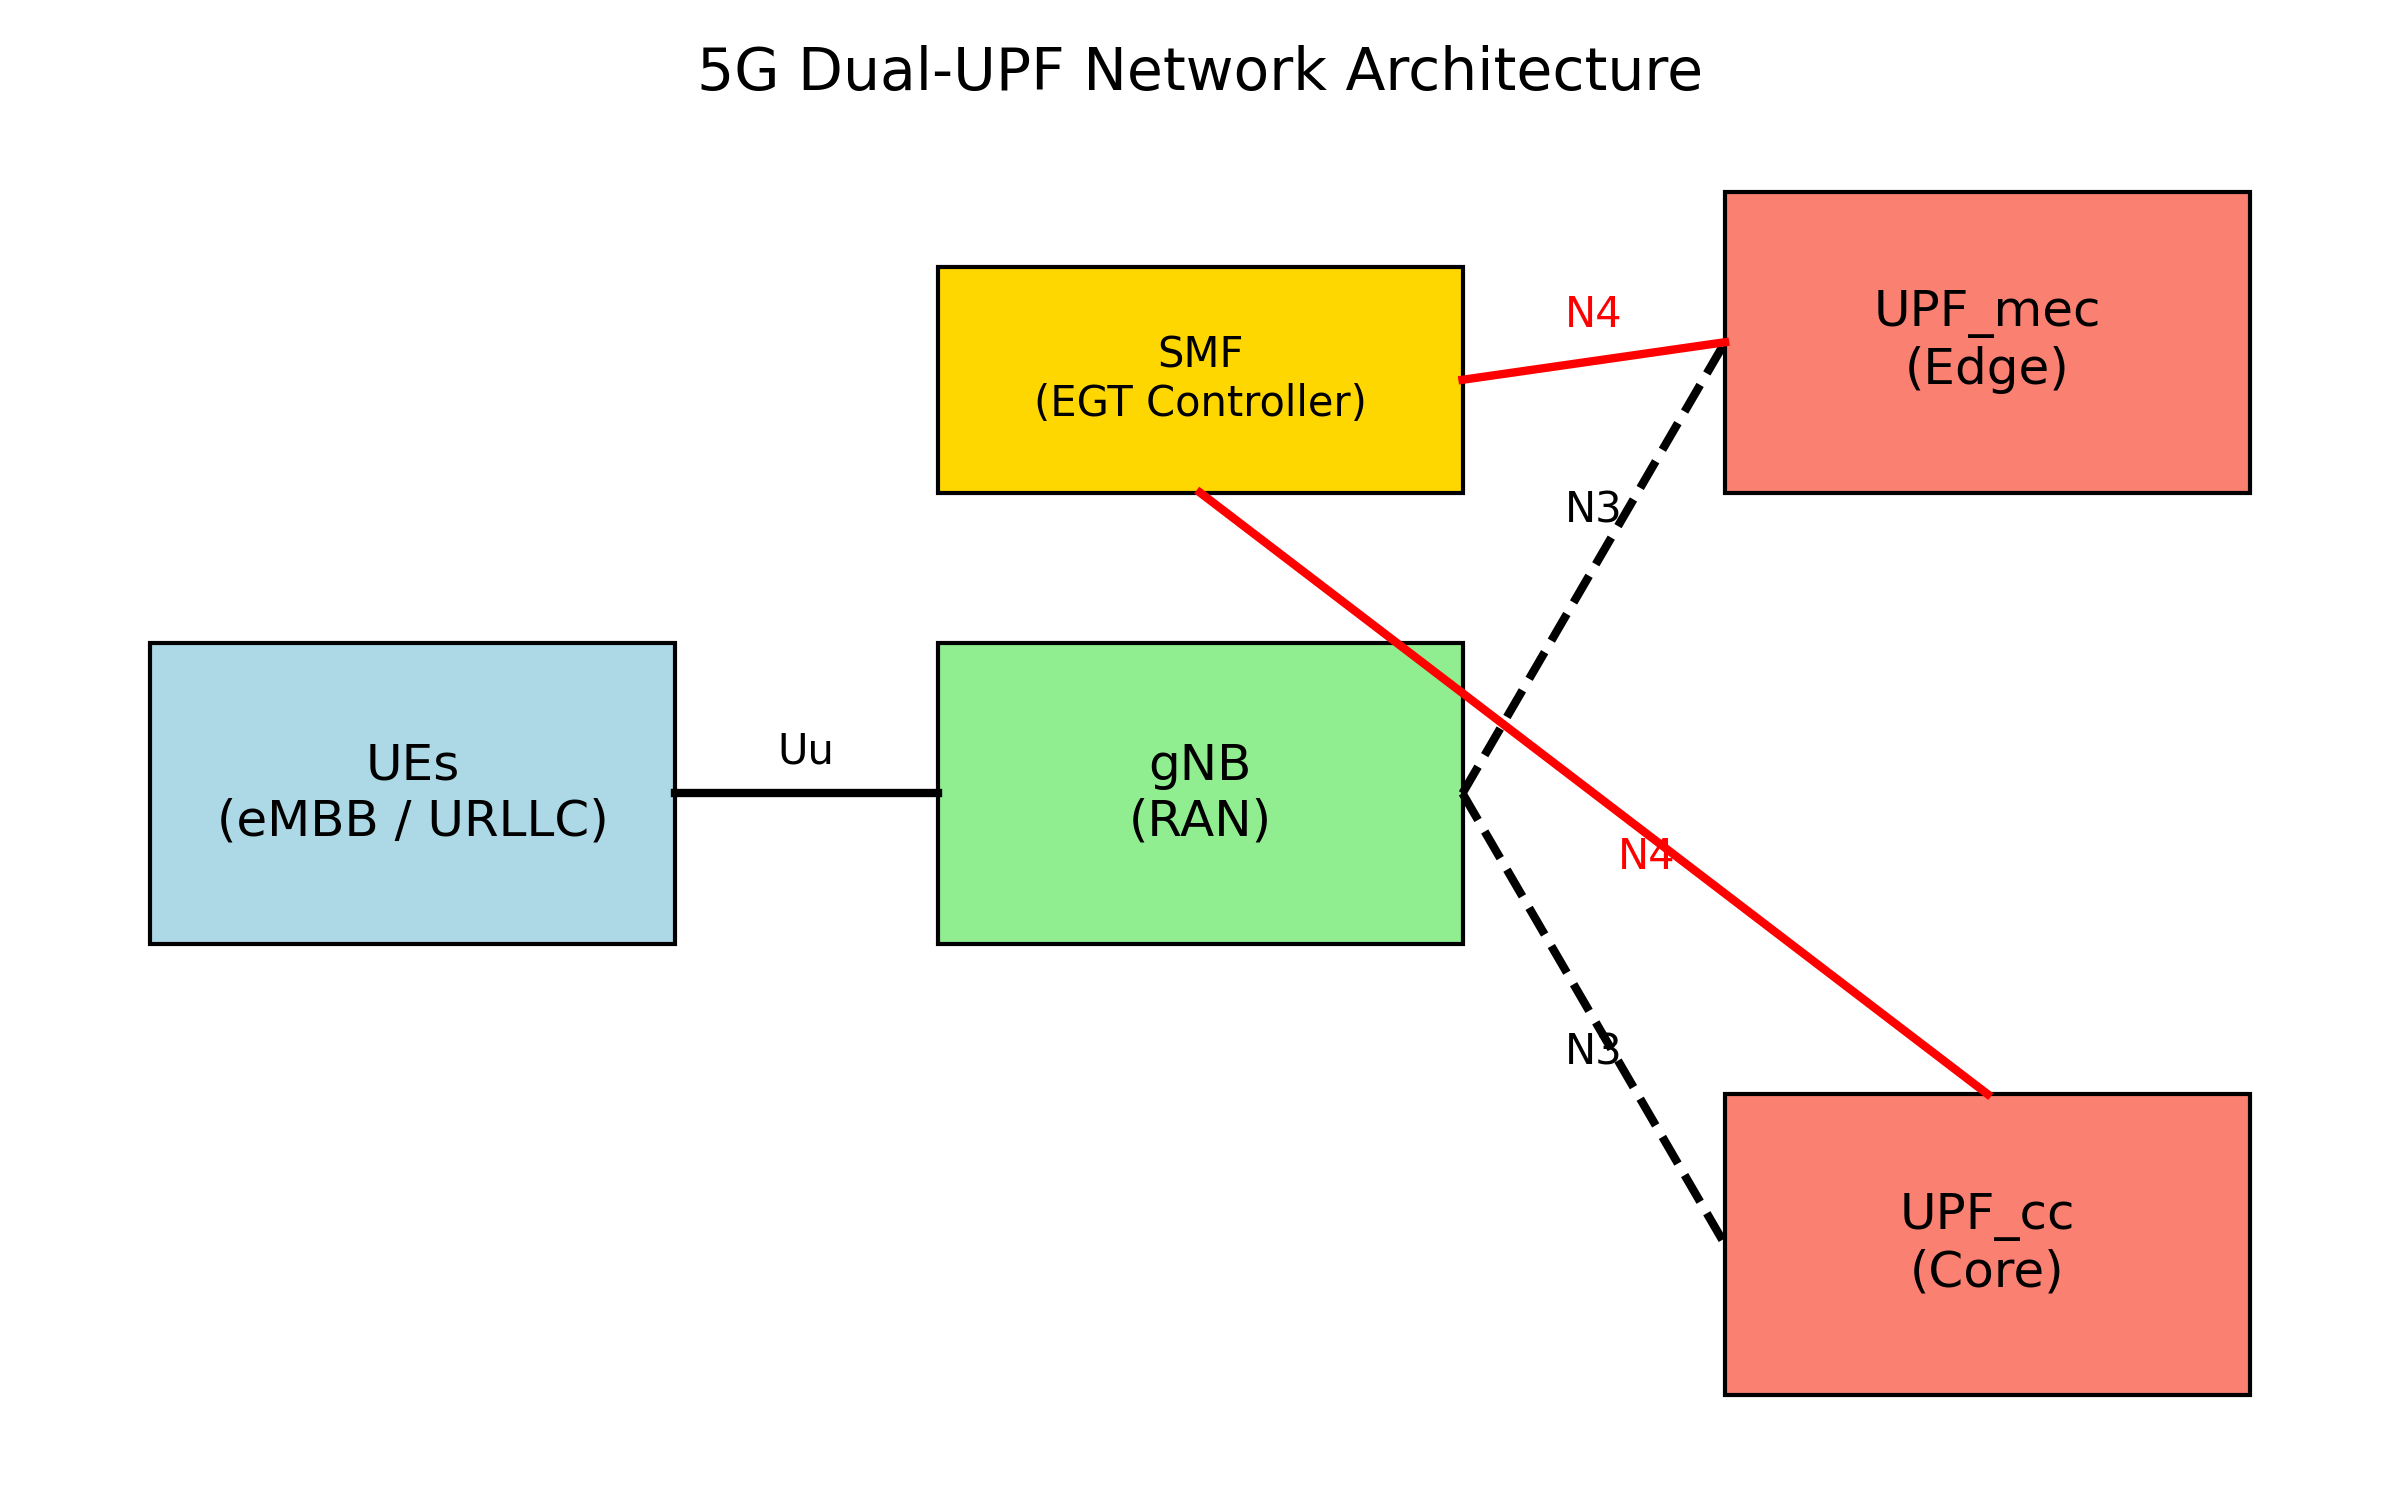
\includegraphics[width=0.45\textwidth]{image1.png}
    \caption{5G dual-UPF network architecture. eMBB and URLLC
    UEs connect to the gNB via the Uu air interface. The gNB
    forwards traffic over N3 to either the MEC edge UPF or the
    central cloud UPF. The SMF steers sessions between both UPFs
    via the N4 control interface.}
    \label{fig:network_architecture}
\end{figure}

As illustrated in Fig.~\ref{fig:network_architecture}, the
proposed topology differentiates between eMBB and URLLC
sessions. Traffic originating from UEs is carried via the
Uu interface to the gNB, then steered over the N3 user-plane
interface to either $\text{UPF}_\text{mec}$ or
$\text{UPF}_\text{cc}$. Session management and UPF selection
are governed by the SMF via the N4/PFCP interface.

The UE population is partitioned into two slice groups
$g \in \{1,2\}$. Group $g=1$ comprises eMBB users
(S-NSSAI: SST=1) who represent the dominant traffic
class at a stadium. eMBB traffic in this scenario
primarily consists of HD video replay consumption,
social media upload, and venue app usage. Active
HD video streaming demands approximately $25$~Mbps per
device~\cite{yaqoob2020survey_360video}, while the
average per-device load in a dense shared-cell
environment, as observed in large-event
deployments, is significantly lower due to scheduler
sharing across concurrent
users~\cite{superbowl_lvii,ericsson_f1_2023}.
We model $\rho_\text{eMBB} = 10$~Mbps as the mean
offered load per eMBB UE under peak conditions, which
is conservative relative to peak single-device rates
but reflects realistic concurrent cell loading.

Group $g=2$ comprises URLLC users (S-NSSAI: SST=2)
supporting latency-sensitive AR/VR overlay services
offloaded to the MEC node. In this deployment, URLLC
sessions serve real-time AR rendering tasks in which
compute-intensive frame processing is handled at the
MEC server and only compressed output is delivered
to headsets, requiring $\rho_\text{URLLC} = 25$~Mbps
per session~\cite{yaqoob2020survey_360video} with a
strict packet delay budget. Both the per-slice
packet delay budgets $\text{PDB}_g$ and 5QI values
are derived from Table~5.7.4-1 of
3GPP~TS~23.501~\cite{3gpp_ts23501} and
TS~22.261~\cite{3gpp_ts22261}: $\text{PDB}_1 = 300$~ms
for eMBB video (5QI~6, non-GBR) and
$\text{PDB}_2 = 10$~ms for URLLC AR/VR rendering
(5QI~83, Delay-Critical GBR)~\cite{3gpp_ts22261}.
The selection of 5QI~83 over more stringent URLLC classes
(e.g.\ 5QI~82, 3~ms PDB, V2X) reflects the perceptual
latency thresholds of AR/VR rendering: human visual
persistence of motion sets a practical bound of
approximately 20~ms~\cite{yaqoob2020survey_360video},
placing the 10~ms PDB well within the perceptible
response envelope. The sub-millisecond targets of
3GPP TS~22.104 (industrial discrete automation) are
not applicable to the consumer AR/VR use case modelled here.
The evaluation covers eMBB and URLLC slices only;
massive Machine Type Communication (mMTC) traffic is excluded
on the basis that its characteristically low per-device
throughput ($\ll 1$~Mbps) exerts negligible UPF selection
pressure relative to the eMBB and URLLC loads modelled here.
All parameters are listed in Table~\ref{tab:params}.

\begin{table}[ht]
\centering
\caption{System, slice, and algorithm parameters}
\label{tab:params}
\renewcommand{\arraystretch}{1.15}
\begin{tabular}{p{1.8cm}p{2.2cm}p{3.6cm}}
\toprule
\textbf{Symbol} & \textbf{Value} &
\textbf{Description and source} \\
\midrule
\multicolumn{3}{l}{\textit{Network topology}} \\
$C_c^\text{mec}$ & 40 cores (2.4~GHz) &
  MEC server capacity (edge-constrained) \\
$C_c^\text{cc}$ & 120 cores (2.4~GHz) &
  Central server capacity \\
% R5-Q5: Changed B_uv from 100 Gbps to >=200 Gbps (ECMP aggregate)
$B_{u,v}$ & $\geq\!200$~Gbps (ECMP aggregate) &
  Core backhaul aggregate capacity via ECMP multi-path;
  S2 operates beyond single-path limits as a deliberate
  stress test$^\ddagger$ \\
$t_{\text{prop}_\text{mec}}$ & 0.25~ms &
  Propagation delay to local UPF \\
$t_{\text{prop}_\text{cc}}$ & 1.0~ms &
  Propagation delay to central UPF \\
\midrule
\multicolumn{3}{l}{\textit{Slice parameters
  (3GPP TS 22.261~\cite{3gpp_ts22261},
   TS 23.501~\cite{3gpp_ts23501})}} \\
$M_1$ & 800 &
  eMBB UE population (SST=1) \\
$M_2$ & 200 &
  URLLC UE population (SST=2) \\
$\rho_\text{eMBB}$ & 10~Mbps &
  Mean per-UE eMBB load at
  peak~\cite{superbowl_lvii,ericsson_f1_2023} \\
$\rho_\text{URLLC}$ & 25~Mbps &
  Per-session AR/VR offload
  load~\cite{yaqoob2020survey_360video} \\
$\text{PDB}_1$ & 300~ms &
  eMBB PDB, 5QI~6~\cite{3gpp_ts23501} \\
$\text{PDB}_2$ & 10~ms &
  URLLC AR/VR PDB,
  5QI~83~\cite{3gpp_ts22261} \\
\midrule
\multicolumn{3}{l}{\textit{UPF delay
  model~\cite{Alevizaki2021upf}}} \\
$k_\text{mec}$ & $4.833\!\times\!10^{-4}$ &
  Processing exponent, local UPF
  (units: Mbps$^{-1}$); calibrated via
  grid search against Fig.~2
  of~\cite{Alevizaki2021upf} \\
$k_\text{cc}$ & $4.833\!\times\!10^{-5}$ &
  Processing exponent, central UPF;
  ratio $k_\text{mec}/k_\text{cc}=10$
  per~\cite{Alevizaki2021upf} \\
\midrule
\multicolumn{3}{l}{\textit{EGT algorithm~\cite{Alevizaki2021upf}}}\\
$\beta$ & 1 &
  Payoff scaling constant \\
$a$ & 1 &
  Review rate upper bound; $a/\beta=1$
  per~\cite{Alevizaki2021upf} \\
$\varepsilon$ & 0.01 &
  Payoff convergence threshold \\
$\Delta t$ & 0.05 &
  Discrete replicator step size \\
\bottomrule
\multicolumn{3}{l}{\footnotesize $^\ddagger$$B_{u,v}$ represents aggregate backhaul
  capacity via ECMP multi-path routing across}\\
\multicolumn{3}{l}{\footnotesize multiple 100~Gbps wavelengths; S2 ($\lambda=10\times$,
  total load 130~Gbps) operates beyond}\\
\multicolumn{3}{l}{\footnotesize single-path limits as a deliberate infrastructure
  stress test.}\\
\end{tabular}
\end{table}

%--------------------------------------------------------------
\subsection{Traffic Dynamics at Mass Events}
\label{sec:traffic}
%--------------------------------------------------------------

A defining characteristic of the stadium scenario is the
pronounced non-stationarity of traffic demand. Real-world
measurements at large events document this pattern
clearly. At Super Bowl LIII, 24~TB of data were
transferred within the stadium alone, with the data
network spiking to 13.06~Gbps during the halftime show
from over 30,000 concurrent mobile
devices~\cite{nokia_live_events}. At Super Bowl~LVII,
a peak Wi-Fi throughput of 25.8~Gbps was recorded,
and the halftime show drove a 450\% increase in
bandwidth usage relative to the pre-show
baseline~\cite{superbowl_lvii}. At the 2023 Formula~1
Grand Prix in Mexico~City, 5G accounted for 40\% of
over 117~TB of total mobile data traffic, with average
5G download speeds of 274~Mbps for connected
users~\cite{ericsson_f1_2023}. These measurements
establish three distinct load phases that our model
must capture. The halftime demand spike is modelled at
$\lambda = 5.5\times$ the pre-spike baseline; a 450\% increase
above the pre-match baseline corresponds to a load multiplier
of $\lambda = 1 + 4.5 = 5.5$~\cite{superbowl_lvii}.
At this multiplier the total offered load is
$(M_1\rho_\text{eMBB} + M_2\rho_\text{URLLC})\,\lambda
= 13~\text{Gbps} \times 5.5 = 71.5~\text{Gbps}$.

% R5-Q10: Added explicit Phase I ramp model description
% R6-Q1: S4 Phase I uses a different lambda ramp (0.509->5.0) from S1 (0.011->1.0);
%         this paragraph describes the standard (S1/S2/S3) ramp only.
\textbf{Pre-match ramp-up (Phase~I).} Spectators enter
the venue over 30--60 minutes. eMBB sessions increase
monotonically as users connect, stream highlights, and
access venue applications. For standard scenarios (S1, S2, S3),
Phase~I is modelled as a linear load ramp with $\lambda$
increasing uniformly from 0.011 to 1.0 over 90 simulation steps
(one step per 20 seconds of the 30-minute ramp), equivalent to
proportionally scaling the active UE population from
approximately 11 to 1,000 concurrent sessions. S4's Phase~I
uses an elevated load ramp ($\lambda$: 0.509 to 5.0$\times$)
reflecting the CC-biased stress initialisation, distinct from
the S1 ramp ($\lambda$: 0.011 to 1.0$\times$). Under standard
load, Phase~I load is moderate and $\text{UPF}_\text{mec}$ can
absorb the majority of sessions with favourable delay; the EGT
equilibrium concentrates sessions at the edge node.

\textbf{Peak-load phase (Phase~II).} At kick-off and
halftime, concurrent eMBB and URLLC sessions generate
the aggregate demand surge documented in field
measurements. Phase~II spans 45~minutes, evaluated at
3~simulation steps per minute, yielding the 135-step
evaluation window reported in the results.
The exponential processing delay model in
Eq.~\eqref{eq:upf_delay_mec}--\eqref{eq:upf_delay_cc}
captures the rapid onset of queuing congestion at
$\text{UPF}_\text{mec}$ as aggregate load approaches
capacity. Rising processing delay reduces the payoff of
the local UPF below the population average, and the
replicator dynamics redistribute sessions to
$\text{UPF}_\text{cc}$. This phase creates the
conditions under which the EGT equilibrium may
transiently lag behind rapid load shifts, motivating
the ML reconfiguration trigger in Section~\ref{sec:future}.

% R5-Q2: Added Phase III lambda profile and residual URLLC violation note
% R6-Q6: Phase III lambda profiles are scenario-specific; corrected to per-scenario values.
\textbf{Post-match dispersal (Phase~III).} Session
counts fall as spectators leave over 20 minutes
(60~simulation steps). Phase~III disperses load from
approximately $\lambda_{\text{Phase~II}}$ down to $0.3\times$,
ramping over 60 steps. For S1/S3/S4 (Phase~II at
$5.5\times$), Phase~III begins at $\lambda \approx 5.0\times$
and decreases to $0.3\times$, producing 199 residual URLLC
violations during the initial dispersal transient. For S2
(Phase~II at $10\times$), Phase~III begins at $\lambda \approx
9.0\times$ and decreases to $0.3\times$, producing 597 residual
URLLC violations during the dispersal transient before load
falls below the infrastructure ceiling. Active
URLLC sessions must not be forcibly re-anchored
during dispersal, as unnecessary PDU session
modifications introduce signalling overhead and
momentary service interruption.

%--------------------------------------------------------------
\subsection{Justification for Evolutionary Game Theory}
\label{sec:egt_justify}
%--------------------------------------------------------------

\textbf{Centralised SMF steering.}
Unlike standard EGT formulations where individual UEs selfishly
optimise their UPF choice, we implement the replicator dynamics
centrally within the SMF to compute optimal population fractions.
This centralised adaptation prevents the massive control-plane
signalling overhead that would occur if 1,000 UEs independently
triggered PDU session renegotiations, while still preserving
the mathematically stable load-balancing properties of the
Nash equilibrium.

The UPF session-steering problem in a stadium environment
has four further properties that make EGT the appropriate
decision framework.

\textbf{Population-scale efficiency.} At peak
load, up to $M_1 + M_2 = 1{,}000$ PDU sessions must be
steered concurrently. Centralised formulations such as
Integer Linear Programming (ILP) are computationally
intractable at this scale and under dynamic
demand~\cite{LeyvaUPC2023}. EGT operates on aggregate
population fractions $\mathbf{x}^g(t)$ rather than
individual sessions, reducing the SMF's per-iteration
complexity from $O(M_g)$ to $O(|\mathcal{S}_g|) = O(2)$
for a two-UPF strategy space~\cite{Alevizaki2021upf}.

\textbf{Non-stationarity.} The three-phase load profile
changes continuously. Unlike static assignment policies,
which require offline re-optimisation to respond to load
changes, the replicator dynamics adapt $\mathbf{x}^g(t)$
continuously to the prevailing payoff landscape without
requiring a global re-solve.

\textbf{Convergence to a stable equilibrium.} The
replicator dynamics converge to a Nash equilibrium at
which all active strategies within each group achieve
equal payoff~\cite{Alevizaki2021upf}. At equilibrium,
neither UPF is overloaded relative to the other given
the current population mix. The current payoff function
(Eq.~\eqref{eq:payoff}) optimises end-to-end delay
rather than PDB margin directly; the relationship between
equilibrium delay and QoS compliance is discussed in
Section~\ref{sec:results}.

\textbf{Low N4 signalling overhead.} The SMF maintains
population state internally; no per-session global state
exchange is required. The algorithm issues N4/PFCP
session modification rules only for newly established
PDU sessions, consistent with the PFCP interaction model
of 3GPP~TS~29.244~\cite{3gpp_ts29244}.

%--------------------------------------------------------------
\subsection{UPF Strategy Space and Population State}
\label{sec:strategy}
%--------------------------------------------------------------

For each group $g \in \{1,2\}$, the strategy set is
$\mathcal{S}_g = \{\text{UPF}_\text{mec},
\text{UPF}_\text{cc}\}$.
The SMF maintains the population state of group $g$ as:
\begin{equation}
    \mathbf{x}^g(t) = \bigl[x_\text{mec}^g(t),\;
    x_\text{cc}^g(t)\bigr], \quad
    x_\text{mec}^g + x_\text{cc}^g = 1
    \label{eq:popstate}
\end{equation}
where $x_i^g(t)$ is the fraction of sessions in group
$g$ currently anchored at $\text{UPF}_i$, computed from
per-UPF session counts reported over N4/PFCP at each
iteration interval $\Delta t$.

%--------------------------------------------------------------
\subsection{Delay Model and Payoff Function}
\label{sec:delay}
%--------------------------------------------------------------

The end-to-end delay for a session in group $g$ anchored
at $\text{UPF}_i$ under load multiplier $\lambda$ is:
\begin{equation}
    d_i^g(\mathbf{x},\lambda) = t_{\text{prop}_i}
    + t_{\text{UPF}_i}^g(\mathbf{x},\lambda)
    \label{eq:delay}
\end{equation}
where $t_{\text{prop}_i}$ is the fixed propagation delay
to $\text{UPF}_i$ and $t_{\text{UPF}_i}^g$ is the
processing and queuing delay, modelled as an exponential
function of offered load following~\cite{Alevizaki2021upf}.

The two UPFs have different resource-sharing assumptions
that match the deployed architecture. The edge
$\text{UPF}_\text{mec}$ operates with dedicated
per-slice processing: only the sessions of group $g$
itself contribute to that group's delay at the edge.
The central $\text{UPF}_\text{cc}$ is a shared node
whose processing load is the aggregate across all groups.
Accordingly:
\begin{align}
    t_{\text{UPF}_\text{mec}}^g(\mathbf{x},\lambda)
      &= \exp\!\bigl(k_\text{mec}\cdot
         \rho_g\,M_g\,x_\text{mec}^g\,\lambda\bigr)
    \label{eq:upf_delay_mec} \\[4pt]
    t_{\text{UPF}_\text{cc}}(\mathbf{x},\lambda)
      &= \exp\!\Bigl(k_\text{cc}\cdot\lambda
         \sum_{g'=1}^{G}\rho_{g'} M_{g'}
         x_\text{cc}^{g'}\Bigr)
    \label{eq:upf_delay_cc}
\end{align}
where $\rho_g$ is the per-UE offered load for slice group
$g$, $M_g$ is the group population, and $k_i$ is a
node-specific exponent whose units are Mbps$^{-1}$.
Note that $t_{\text{UPF}_\text{cc}}$ carries no group
superscript because the central UPF delay is identical
for all groups at a given load point.

The exponential form captures the superlinear onset of
queuing delay as utilisation approaches the node's
processing capacity. Since $k_\text{mec} \gg k_\text{cc}$,
$\text{UPF}_\text{mec}$ degrades faster under load than
$\text{UPF}_\text{cc}$, reproducing the edge--core
capacity asymmetry characteristic of stadium
deployments~\cite{nokia_live_events}.

The node-specific exponents are calibrated via grid search
to reproduce the reference equilibrium fractions of Fig.~2
in~\cite{Alevizaki2021upf}, using the reference parameters
$M_1=130$, $M_2=70$, $\rho=100$~Mbps. The calibrated
values $k_\text{mec} = 4.833\times10^{-4}$~Mbps$^{-1}$
and $k_\text{cc} = 4.833\times10^{-5}$~Mbps$^{-1}$
reproduce the published result to within 0.1\%:
$G_1\text{@MEC} = 17.82\%$ (reference: $\approx 17.8\%$)
and $G_2\text{@MEC} = 31.97\%$ (reference: $\approx 32.0\%$)
in 231 iterations. The 10:1 exponent ratio is preserved
per~\cite{Alevizaki2021upf}. Empirical validation against
physical testbed measurements is left for future work.

% R6-Q8: Added constraint verification and exp(0) baseline explanation
At zero load, the delay model yields a 1~ms processing baseline
($\exp(0) = 1$), representing the minimum pipeline latency inherited
from the optical switching calibration of Alevizaki~et~al.; the
review rate constraint $a/\beta > u_i$ is verified satisfied for all
scenarios, with maximum observed payoff $u_\text{max} = 0.783
< a/\beta = 1.0$.

While Alevizaki~et~al.\ use a single shared delay formula for
both UPFs, we adopt a dedicated-MEC model for the edge UPF, in
which only the sessions of group $g$ contribute to that group's
MEC processing delay. This reflects the 3GPP~TS~23.501 network
slicing architecture, including the QoS flow enforcement framework
of Section~5.7~\cite{3gpp_ts23501}, where per-S-NSSAI resource
isolation at the edge is a core requirement for stadium
deployments with strict URLLC guarantees. The central UPF remains
shared across all groups, consistent with the reference model.

We note that the $k$ parameters, originally derived from optical
switching hardware, are utilised here as generic capacity
constraints to preserve the 10:1 cloud-to-edge ratio and test
the steering logic's stability. In a physical software UPF
deployment, extreme overload would result in packet drops and
session rejections rather than unbounded exponential queuing delay.

The payoff for sessions in group $g$ anchored at
$\text{UPF}_i$ is the inverse end-to-end delay:
\begin{equation}
    u_i^g(\mathbf{x},\lambda) =
    \frac{1}{d_i^g(\mathbf{x},\lambda)}
    \label{eq:payoff}
\end{equation}

It is important to note that this payoff function minimises
end-to-end delay but is blind to discrete per-slice PDB thresholds:
the controller cannot distinguish the 300~ms eMBB boundary from
the 10~ms URLLC boundary. When hardware capacity prevents the
equilibrium delay from falling below $\text{PDB}_2$, the algorithm
cannot compensate through steering alone. A PDB-margin payoff of
the form $u_i^g = \text{PDB}_g / d_i^g(\mathbf{x},\lambda)$ would
drive URLLC traffic more aggressively toward lower-delay nodes and
is identified as a critical direction for future work.

The PDB thresholds $\text{PDB}_g$ serve as monitoring
indicators: a session is counted as a latency violation
when $d_i^g(\mathbf{x},\lambda) > \text{PDB}_g$.
The instantaneous violation count $L_t$ is reported as
a QoS compliance metric and is intended to serve as an
input to the ML trigger described in
Section~\ref{sec:future}, but does not feed back into
the payoff function or alter the steering logic in the
current implementation.

%--------------------------------------------------------------
\subsection{EGT Replicator Dynamics}
\label{sec:egt}
%--------------------------------------------------------------

The SMF adapts session-to-UPF assignments by running the
EGT replicator dynamics of~\cite{Alevizaki2021upf}.
The review rate for sessions in group $g$ at
$\text{UPF}_i$ is:
\begin{equation}
    r_i^g(\mathbf{x},\lambda) =
    a - \beta\,u_i^g(\mathbf{x},\lambda),
    \quad \beta > 0,\quad
    \frac{a}{\beta} > u_i^g(\mathbf{x},\lambda)
    \label{eq:revrate}
\end{equation}
Sessions with high payoff (low delay) are reviewed less
frequently, stabilising their assignment. Population
fractions evolve according to:
% R6-Q4: Added footnote clarification about the (u_j - ubar) form vs standard replicator.
%         Both forms share the same interior Nash equilibrium; they differ only in
%         convergence trajectory speed.
\begin{equation}
    \dot{x}_i^g(t) = \beta\Bigl(u_j^g(\mathbf{x},\lambda)
    - \bar{u}^g(\mathbf{x},\lambda)\Bigr)x_i^g, \quad
    \bar{u}^g = \sum_i x_i^g\,u_i^g(\mathbf{x},\lambda)
    \label{eq:replicator}
\end{equation}
where $u_j^g(\mathbf{x},\lambda)$ denotes the payoff of
an alternative UPF strategy $j \in \mathcal{S}_g$,
$j \neq i$, chosen at random by the reviewing agent
under the pairwise comparison protocol
of~\cite{Alevizaki2021upf}.\footnote{Following the pairwise
comparison protocol of~\cite{Alevizaki2021upf}, the replicator
uses $(u_j - \bar{u})\cdot x_i$ as a convenient equivalent
form; both this and the standard form $(u_i - \bar{u})\cdot x_i$
converge to the same interior Nash equilibrium
$u_\text{mec}^g = u_\text{cc}^g$, differing only in the speed
of the convergence trajectory.}
The continuous-time system converges to the interior
Nash equilibrium $u_\text{mec}^g = u_\text{cc}^g$ for
each group $g$~\cite{Alevizaki2021upf}.

In the discrete-time implementation, the SMF integrates
Eq.~\eqref{eq:replicator} with step size $\Delta t = 0.05$
up to a maximum of 2{,}000 iterations per convergence
call. Two stopping criteria are applied in conjunction:
(i) the maximum per-group payoff deviation falls below
$\varepsilon = 0.01$, i.e.\
$\max_i |u_i^g - \bar{u}^g| < \varepsilon$ for all
interior-strategy groups; and (ii) the maximum
per-element strategy change $\max_{g,i}|x_i^g{}^{(t+1)}
- x_i^g{}^{(t)}| < 2\times10^{-5}$, which detects
convergence to a boundary equilibrium where one UPF
carries zero sessions. Groups with all sessions on a
single UPF (a boundary state) are skipped in the payoff
check, as the payoff equality condition is not applicable
at the boundary.
% R5-Q8: Clarified that the two stopping criteria apply
% independently per slice group
The algorithm applies the payoff criterion independently
per slice group. At the reported S1 equilibrium, the
URLLC payoff gap is 0.0032 ($< \varepsilon$), satisfying
criterion~(i); eMBB terminates on the strategy-change
criterion~(ii) ($|\Delta x| < 2\times10^{-5}$),
reflecting convergence to a boundary-adjacent state where
the gradient is too small to move further.

Established sessions are not re-anchored mid-flight
within an iteration to avoid service interruption; the
redistribution applies to new establishments only.

% ------------------------------------------------------------------
% FLOWCHART FIGURES
% ------------------------------------------------------------------

\begin{figure*}[t]
    \centering
    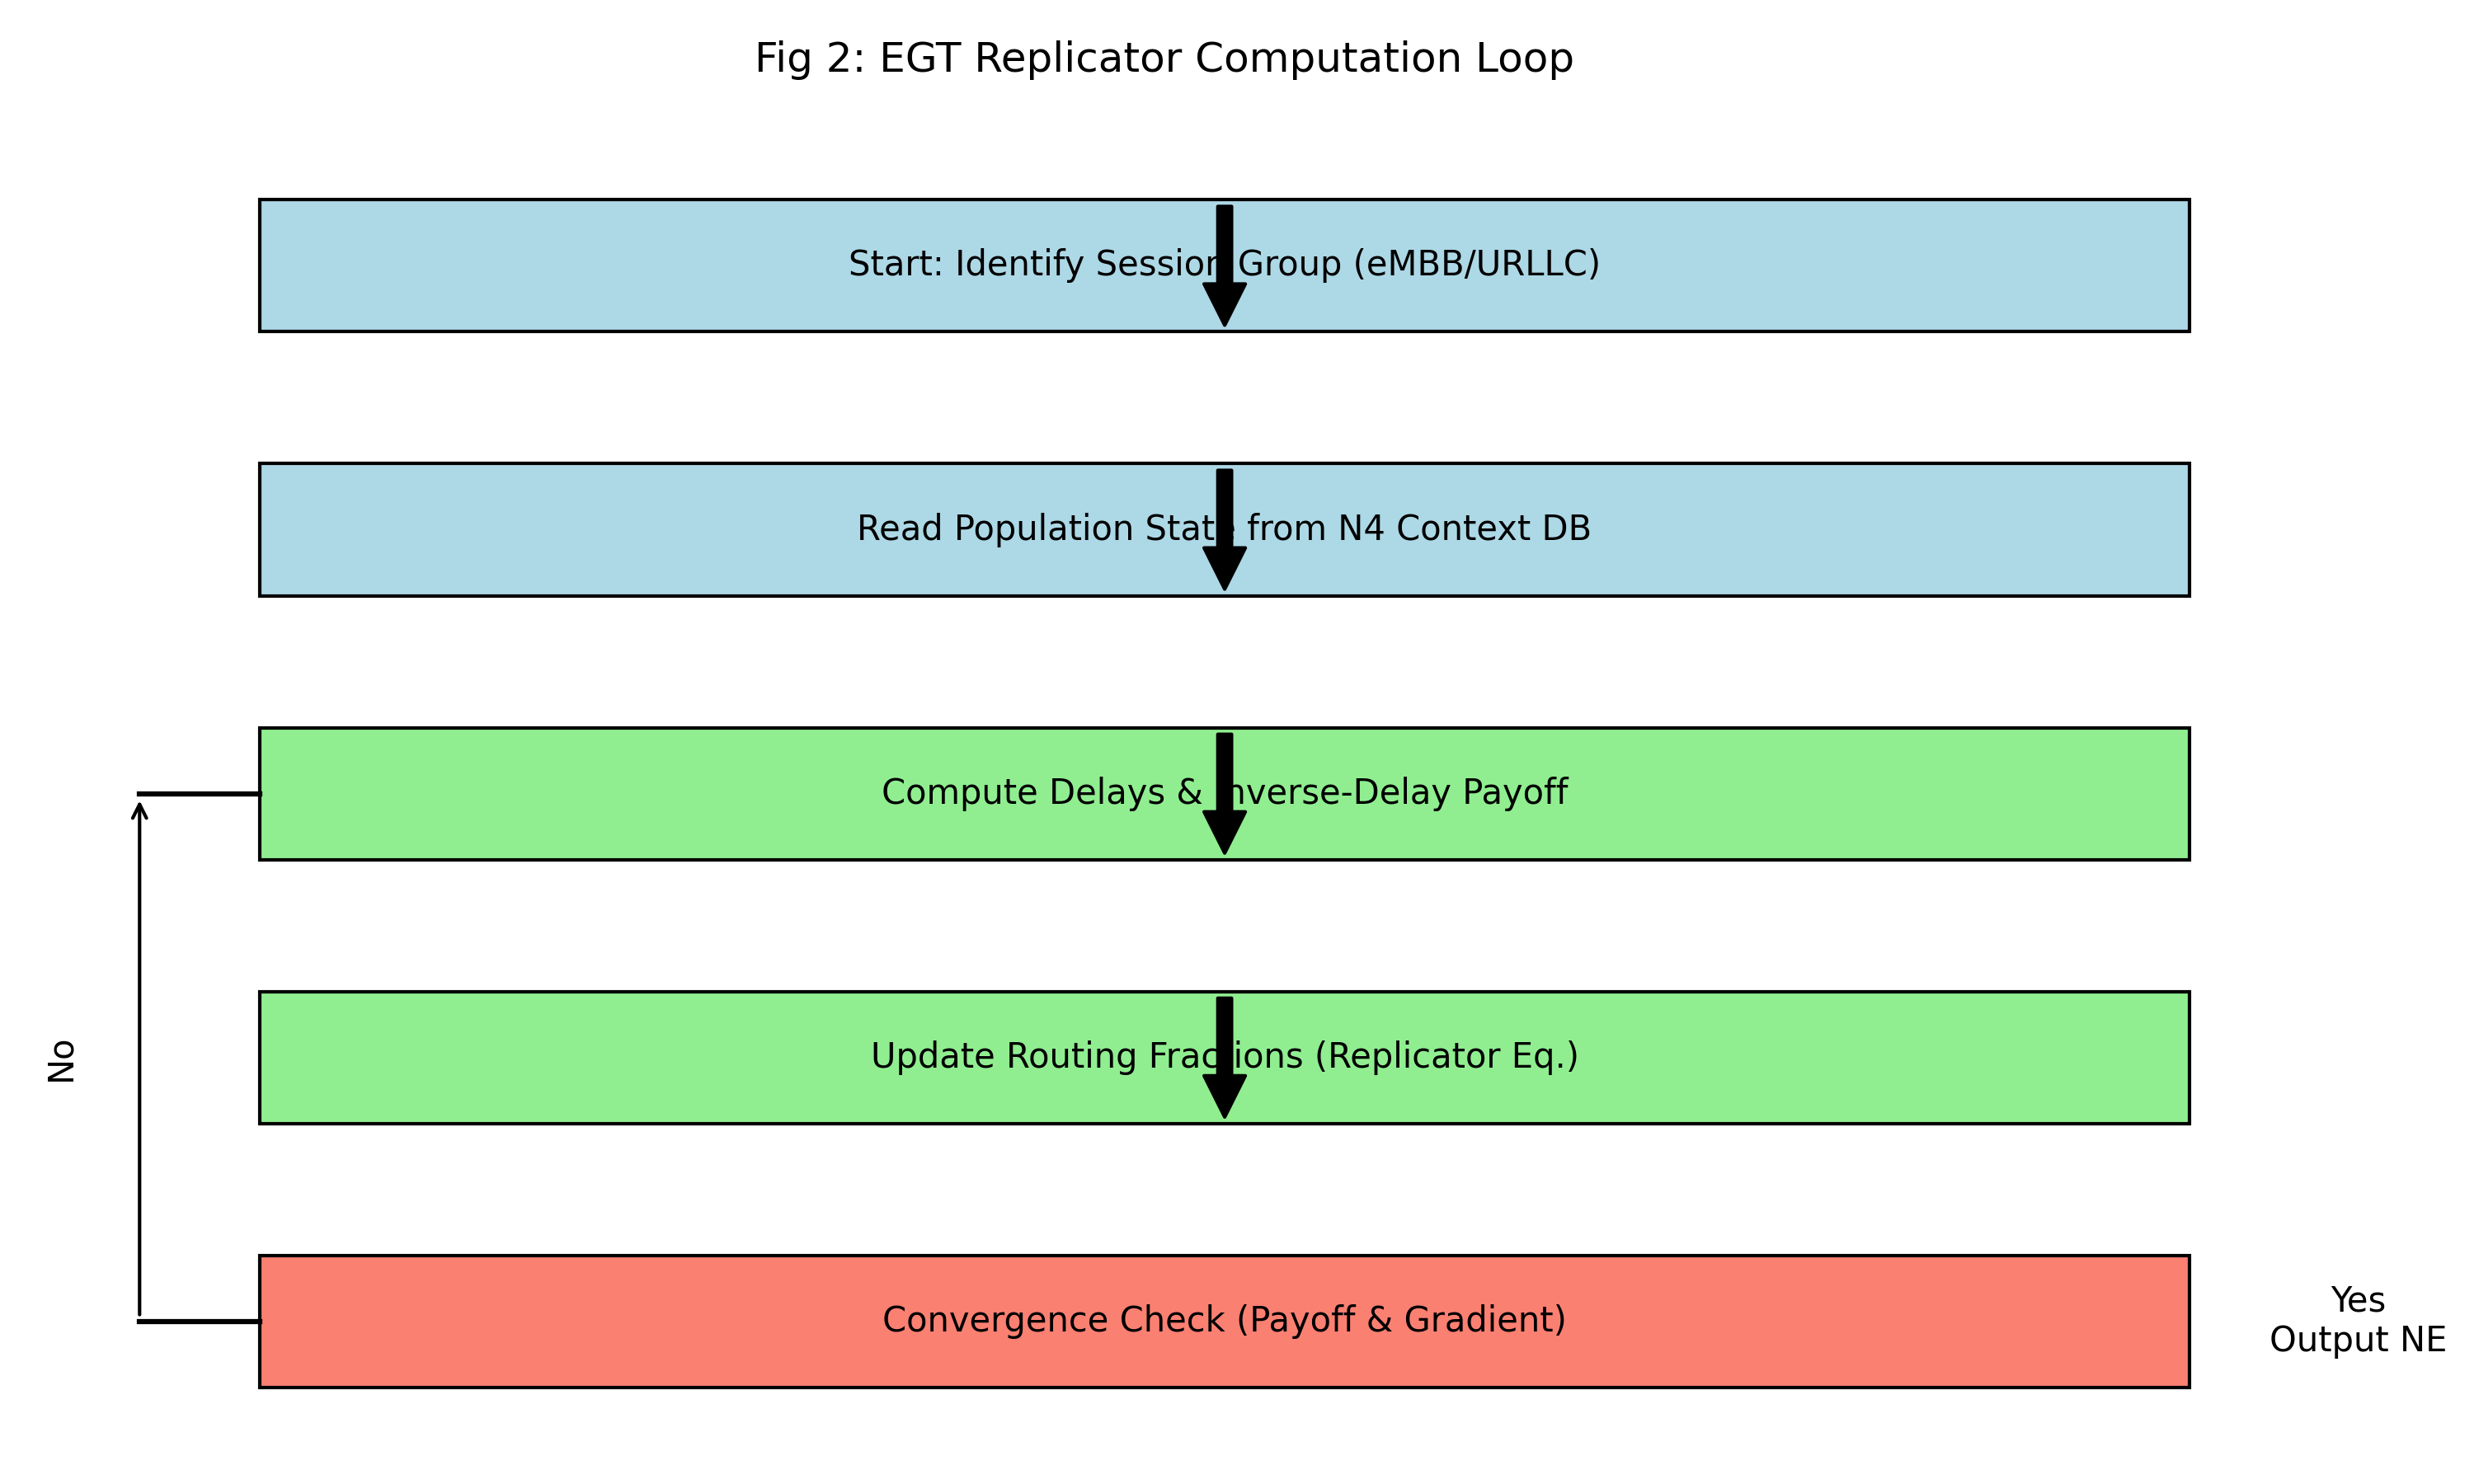
\includegraphics[width=\textwidth, trim={0 10pt 0 10pt}, clip]{flowchart1.png}
    \caption{EGT replicator computation loop (inner loop, Fig.~2).
    On each invocation, the SMF identifies the slice group $g$ of
    the arriving PDU session, reads the current population state
    $\mathbf{x}^g$ from N4/PFCP session counts, and iterates
    Eq.~\eqref{eq:replicator}: computing UPF processing delays
    (Eqs.~\eqref{eq:upf_delay_mec}--\eqref{eq:upf_delay_cc}),
    end-to-end delays (Eq.~\eqref{eq:delay}), inverse-delay
    payoffs (Eq.~\eqref{eq:payoff}), and the mean payoff
    $\bar{u}^g$, then applying the replicator step
    $\Delta x_i = \beta(u_j - \bar{u}^g)x_i\,\Delta t$.
    Iteration continues until both the payoff-deviation criterion
    ($\max_i|u_i^g - \bar{u}^g| < \varepsilon$) and the
    strategy-stability criterion
    ($\max_{g,i}|\Delta x_i| < 2\!\times\!10^{-5}$) are
    satisfied simultaneously, at which point the Nash-equilibrium
    fractions $x_\text{mec}^g$ and $x_\text{cc}^g$ are output
    to the session dispatch loop (Fig.~\ref{fig:flowchart_dispatch}).}
    \label{fig:flowchart_egt}
\end{figure*}

\begin{figure*}[t]
    \centering
    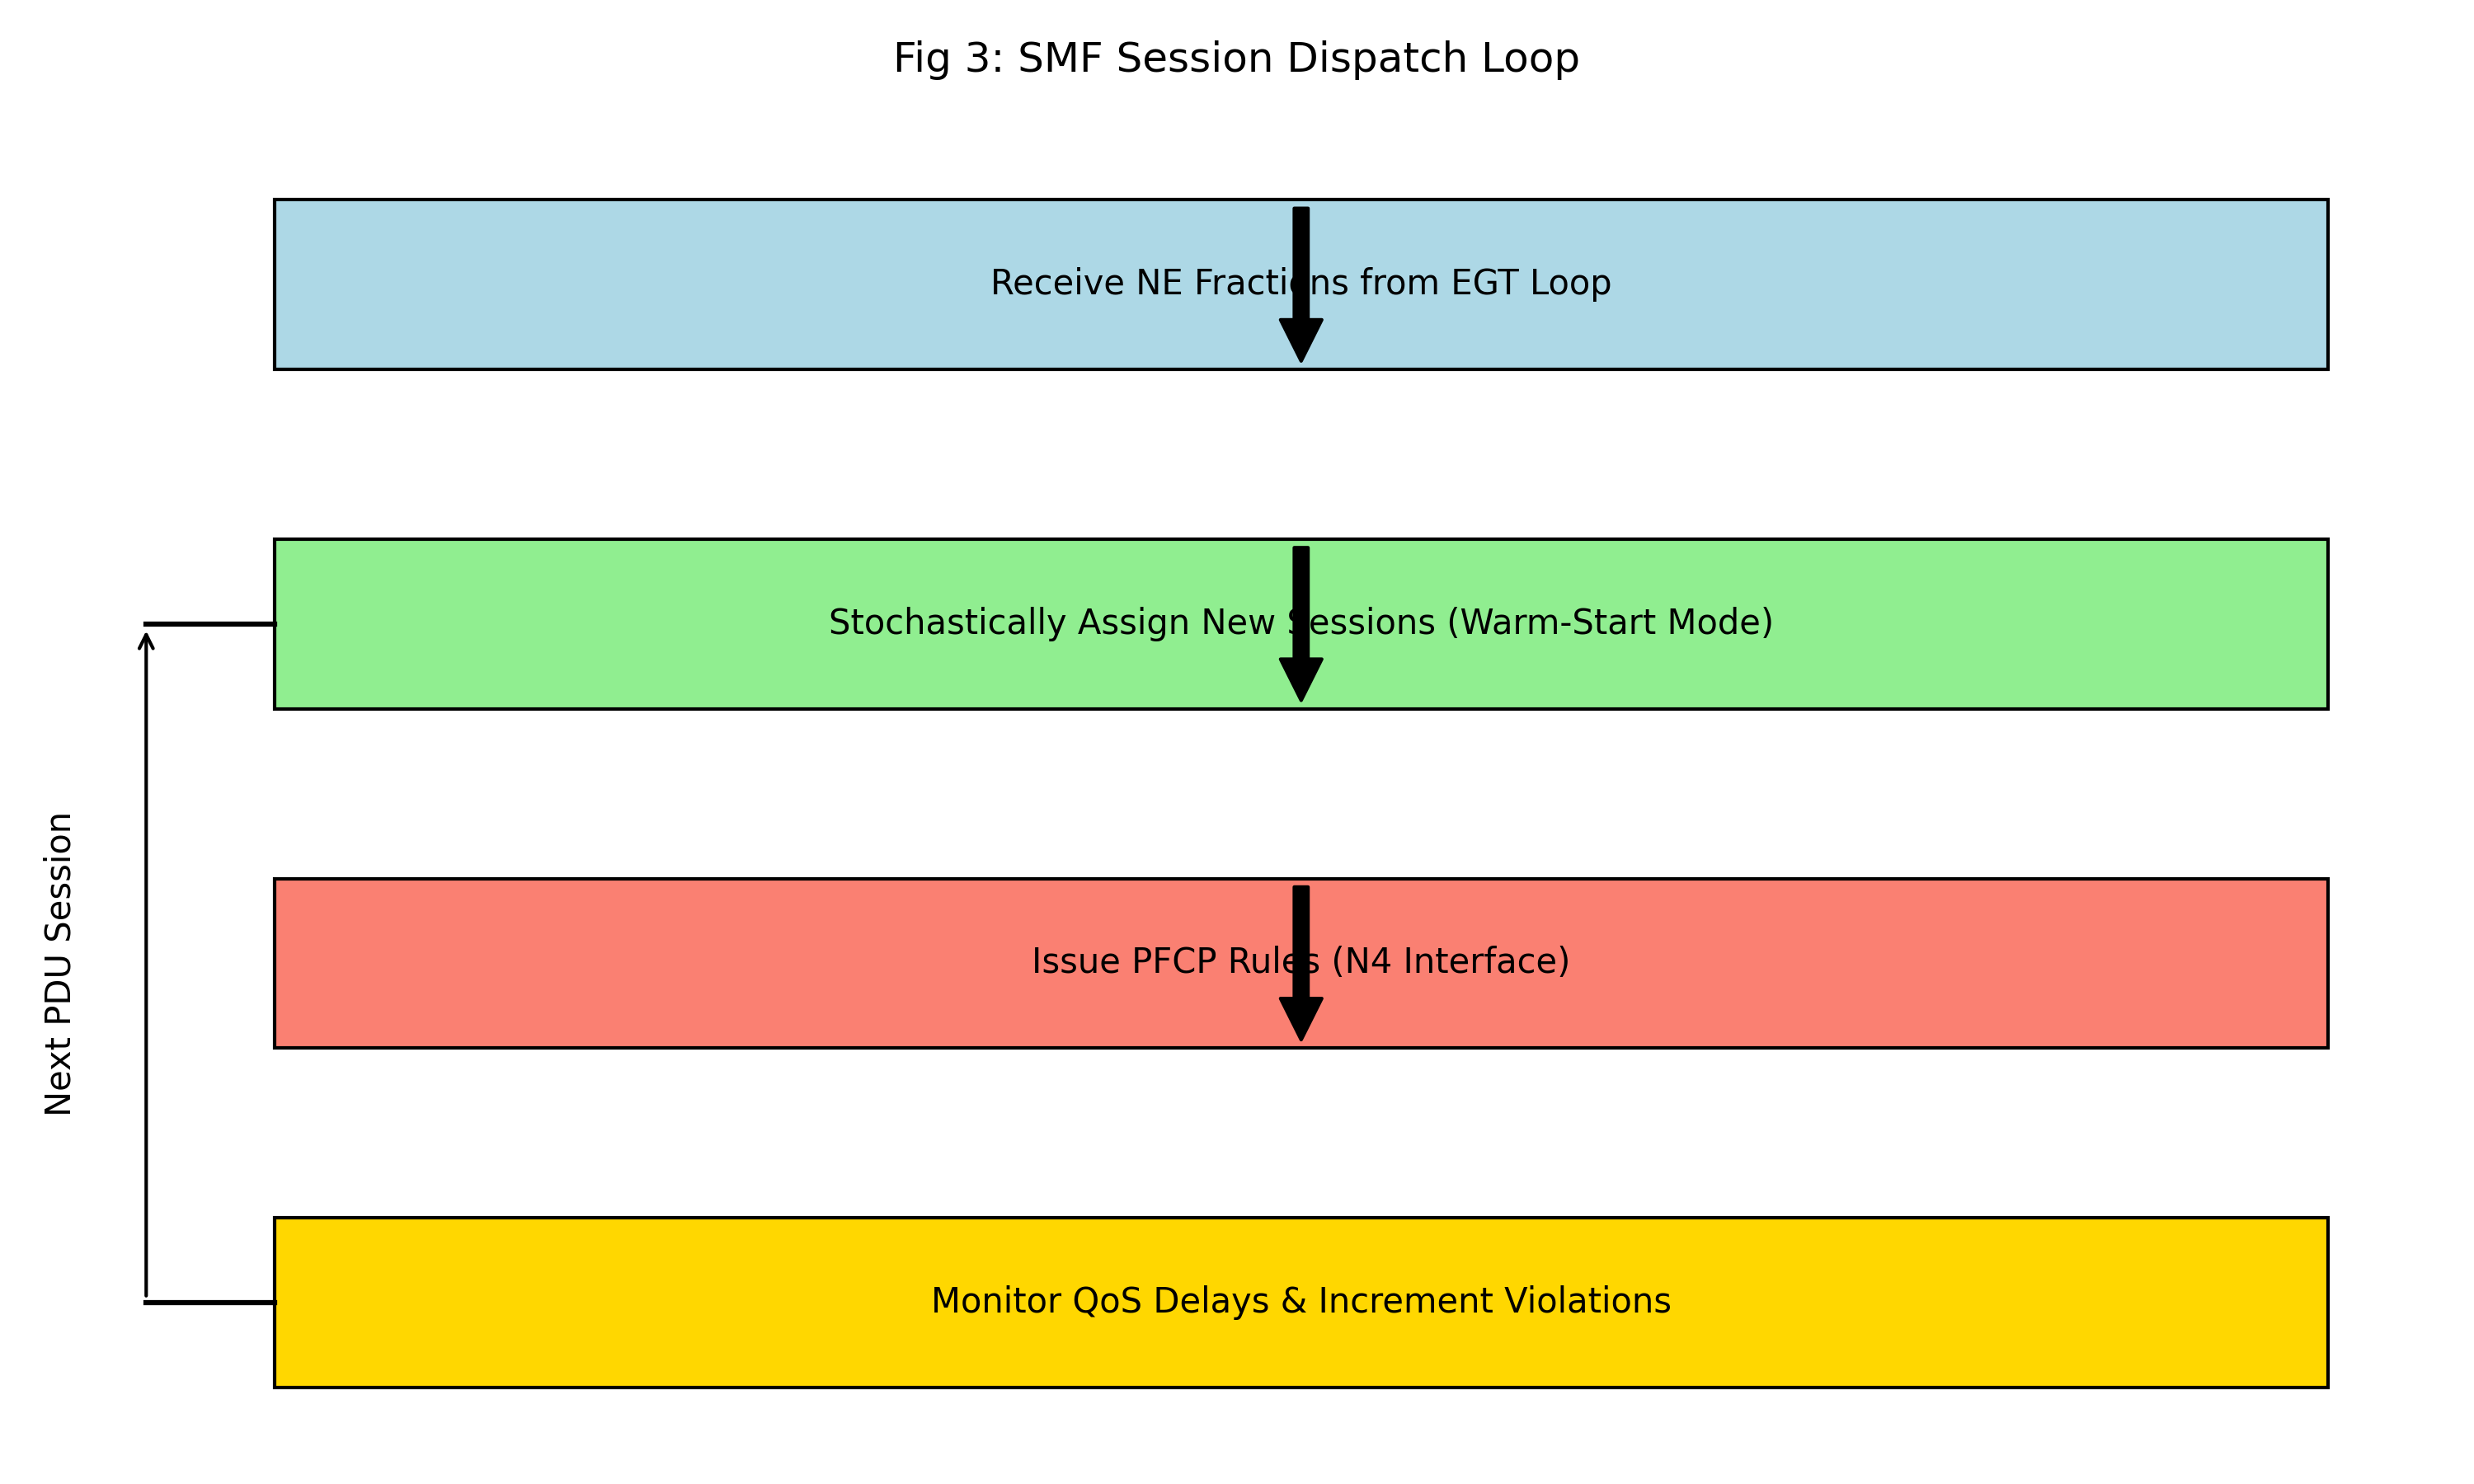
\includegraphics[width=\textwidth, trim={0 10pt 0 10pt}, clip]{flowchart2.png}
    \caption{SMF session dispatch loop (outer loop, Fig.~3).
    Given the equilibrium fractions $x_\text{mec}^g$ and
    $x_\text{cc}^g$ from the EGT computation loop
    (Fig.~\ref{fig:flowchart_egt}), the SMF selects the
    initialisation mode: in warm-start mode the previous
    population state is carried forward as the starting point,
    avoiding cold-start numerical traps under gradual load
    transitions; otherwise fractions are reset to
    $x_\text{mec} = x_\text{cc} = 0.5$. Each new PDU session
    is stochastically assigned to $\text{UPF}_\text{mec}$ or
    $\text{UPF}_\text{cc}$ according to $x_\text{mec}^g$, and
    the corresponding N4/PFCP anchor rule is issued. Session
    delay $d_i^g$ is continuously monitored; whenever
    $d_i^g > \text{PDB}_g$ the violation counter $L_t$ is
    incremented for downstream ML-trigger input. On a load-phase
    transition the EGT computation loop is re-invoked to
    recompute equilibrium fractions; otherwise monitoring
    continues for the active session.}
    \label{fig:flowchart_dispatch}
\end{figure*}

% ------------------------------------------------------------------
% END FLOWCHART BLOCK
% ------------------------------------------------------------------

%--------------------------------------------------------------
\subsection{Emulation Prototype}
%--------------------------------------------------------------

The methodology is validated on an OpenAirInterface~(OAI)
emulation testbed comprising OAI~CN5G as the 5G standalone
core, which natively supports multi-UPF deployment and
network slicing via its NSSF-enabled configuration
(AMF, SMF, UPF, NRF, UDM, AUSF, UDR,
NSSF)~\cite{oai_cn5g}. Two OAI~UPF instances are
deployed as separate containerised processes, each with
distinct GTP-U N3 tunnel endpoints and N6 interface
bindings, registered to the NRF and associated with the
SMF via PFCP over N4. Two network slices are provisioned
with S-NSSAIs SST=1 (eMBB, 5QI~6) and SST=2
(URLLC, 5QI~83), with per-slice QoS flow parameters
drawn from Table~5.7.4-1 of
3GPP~TS~23.501~\cite{3gpp_ts23501}.

The EGT controller is implemented in Python and runs
alongside the OAI~CN5G stack. It reads per-UPF session
counts to compute $\mathbf{x}^g(t)$ and updates the
population state at each iteration. A Bidirectional LSTM
(BLSTM) predictor module is prototyped for future
integration into the control loop; its evaluation is
addressed in Section~\ref{sec:future}.

Traffic load traces emulate the three event phases of
Section~\ref{sec:traffic}: a 30-minute ramp-up from zero
to $M_1 + M_2$ concurrent sessions, a 45-minute peak
phase with a halftime demand spike at $\lambda = 5.5\times$
(corresponding to the 450\% increase reported
in~\cite{superbowl_lvii}), and a 20-minute dispersal
phase. An extreme stress scenario uses $\lambda = 10\times$
to characterise infrastructure saturation limits.

\section{System Implementation and Architectural Considerations}
\label{sec:implementation}

To validate the EGT steering logic under high load, we
developed an emulation testbed using OpenAirInterface
(OAI) and a modified version of the \texttt{gnbsim}
emulator. Supporting 1,000 concurrent PDU sessions
required architectural changes to the standard
per-UE processing model.

\subsection{High-Performance User-Plane Multiplexing}

Standard mobile simulators typically spawn independent
goroutines for each User Equipment, leading to resource
contention at high densities. We addressed this by
re-engineering the emulator's user-plane architecture
into a multiplexed engine using shared
\texttt{sharedEncap} and \texttt{sharedDecap} loops with
$O(1)$ lookup maps---specifically \textit{IpToCamper}
and \textit{TeidToCamper}---to route traffic. This
allows the system to identify the correct UE context
and GTP tunnel parameters for any incoming packet in
constant time, enabling the testbed to sustain the
session volume required by the stadium scenario.
It should be noted that all 1,000 UE sessions are
multiplexed through a single virtual gNB instance;
this differs from a physical multi-cell deployment and
constitutes a simplification in the emulation fidelity.
The single-gNB assumption eliminates inter-cell handover
dynamics (X2/Xn path switching and the associated N2-based
PDU session continuity procedures) that would be present
in a real stadium RAN. This is a fundamental scope
limitation of the current emulation, and physical
multi-cell validation remains a high priority for
future work.

\subsection{EGT Controller Integration}
\label{sec:controller_integration}

The EGT controller retrieves session counts via the
N4/PFCP interface using Session Report messages and
utilises the O1 interface for management-plane telemetry.
At each iteration, the controller uses per-UPF session
counts to compute the population state $\mathbf{x}^g(t)$.
When live SMF data is available, this ensures the
population state reflects actual PDU session anchor
distribution rather than purely mathematical projection.
In scenarios where the SMF interface was not reachable
during evaluation, the controller operated in model-only
mode, and results are reported accordingly.

\section{Results and Discussion}
\label{sec:results}

The emulation successfully provisioned all 1,000 UE contexts
with a 100\% PDU session establishment rate via the multiplexed
gnbsim engine with $O(1)$ GTP-U lookup maps, confirming
the feasibility of high-density emulation on standard hardware.

The EGT steering controller is evaluated across four traffic
scenarios (S1--S4) against a static 50/50 baseline partition.
All scenarios use the dedicated-UPF delay model and pure
replicator dynamics of Alevizaki~et~al.~\cite{Alevizaki2021upf}.
At peak Phase~II load ($5.5\times$ multiplier), the total offered
load is $(800 \times 10 + 200 \times 25) \times 5.5 = 71.5$~Gbps.
eMBB violations are counted over 108,000 eMBB UE-steps
($M_1 \times 135$) within Phase~II; URLLC violations are counted
over 27,000 URLLC UE-steps ($M_2 \times 135$) within Phase~II,
except for Scenario~S4, which spans all 285 simulation steps
(57,000 URLLC UE-steps, $M_2 \times 285$) due to Phase~I
violations arising from the 95\% CC-bias initial condition under
the elevated Phase~I load ramp ($\lambda$: 0.509 to 5.0$\times$),
% R5-Q3: Updated S4 denominator and S2 note; corrected to reflect S4 spans 285 steps
% R6-Q1: Added explicit Phase I lambda range for S4
as noted in Table~\ref{tab:stadium_results}.

% R6-Q9: Added scenario definition table per reviewer request
\begin{table}[ht]
\centering
\caption{Scenario Definition: Phase~I/II/III Parameters and Initialisation Conditions}
\label{tab:scenario_def}
\renewcommand{\arraystretch}{1.15}
\begin{tabular}{p{1.5cm}p{0.8cm}p{1.3cm}p{1.0cm}p{0.7cm}p{0.7cm}}
\toprule
\textbf{Scenario} & \textbf{$\lambda$ Ph.II} & \textbf{Ph.I $\lambda$ range} &
  \textbf{Ph.II Init} & \textbf{$x_\text{eMBB}$ start} & \textbf{$x_\text{URLLC}$ start} \\
\midrule
S1 Standard       & 5.5$\times$ & 0.011$\to$1.0 & Warm        & 0.189 & 0.309 \\
S2 Extreme Spike  & 10.0$\times$ & 0.011$\to$1.0 & Warm        & 0.170 & 0.278 \\
S3 MEC-Biased     & 5.5$\times$ & 0.011$\to$1.0 & Cold ($x\!=\!0.90$) & 0.900 & 0.900 \\
S4 CC-Biased      & 5.5$\times$ & 0.509$\to$5.0 & Warm (elev.) & 0.143 & 0.231 \\
\bottomrule
\multicolumn{6}{l}{\footnotesize Phase~III $\lambda$ range: S1/S3/S4: 5.0$\to$0.3$\times$;
  S2: 9.0$\to$0.3$\times$.} \\
\multicolumn{6}{l}{\footnotesize S3 Phase~II init: manual cold-start at $x_\text{mec}=0.90$
  for both slices, overriding Phase~I warm-start.} \\
\end{tabular}
\end{table}

%--------------------------------------------------------------
\subsection{Model Validation Against Reference Equilibrium}
%--------------------------------------------------------------

Before evaluating stadium scenarios, the replicator dynamics
are validated against Fig.~2 of Alevizaki~et~al.~\cite{Alevizaki2021upf}
using the reference parameters ($M_1=130$, $M_2=70$,
$\rho=100$~Mbps). The simulator converges in 231~iterations to:
\begin{equation*}
  G_1\text{@MEC} = 17.82\%,\quad G_2\text{@MEC} = 31.97\%
\end{equation*}
against reference targets of $\approx 17.8\%$ and $\approx 32.0\%$
respectively, confirming that the calibrated parameters
$k_\text{mec} = 4.833\times10^{-4}$ and $k_\text{cc} = 4.833\times10^{-5}$
faithfully reproduce the published result.

%--------------------------------------------------------------
\subsection{Multi-Scenario Performance at Peak Load}
%--------------------------------------------------------------

Table~\ref{tab:stadium_results} summarises the key metrics
at the peak load point of each scenario.

\begin{table*}[t]
\centering
% R5-Q3: Updated caption and footnotes to reflect S4 spanning 285 steps (57,000 UE-steps)
%         and corrected violation rate to 77.2%; S2 footnote retained for full-timeline tracking.
% R6-Q2: S2 URLLC Vio corrected to 26,467 (Phase II only, consistent with eMBB window);
%         597 Phase III residual violations moved to footnote.
% R7-Q1: Clarified Transient Iters as static cold-start benchmark
\caption{EGT Steering Performance at Peak Phase~II Load (1,000 UEs,
         $\lambda=5.5\times$ except S2).
         eMBB violations (S1, S2, S3): cumulative over 108,000 eMBB UE-steps
         ($M_1 \times 135$, Phase~II window).
         URLLC violations (S1, S2, S3): cumulative over 27,000 URLLC UE-steps
         ($M_2 \times 135$, Phase~II window).
         S4 violations: cumulative over the full 285-step event timeline
         (57,000 URLLC UE-steps; $M_2 \times 285$) due to Phase~I
         violations arising from the 95\% CC-bias initial condition
         (Phase~I rate: 94.2\%, Phase~II rate: 99.5\%).
         URLLC Phase~II compliance for S1: 2.5\%
         ($(27{,}000 - 26{,}316)/27{,}000$) --- confirming
         an infrastructure ceiling independent of steering policy.
         Note: S1 and S4 report different equilibrium fractions
         despite identical load because the discrete $\varepsilon$-stopping
         criterion halts on opposite edges of the $\varepsilon$-ball depending
         on the initialisation trajectory; the true Nash equilibrium point
         is the same for all $5.5\times$ scenarios.
         Transient~Iters for S1, S3, S4: theoretical static cold-start convergence
         count (from a neutral 50/50 state), providing a baseline benchmark distinct
         from the dynamic warm-start 1-iteration tracking reported in the text.
         For S2: per-step warm-start tracking count
         (see Section~\ref{sec:key_findings}).}
\label{tab:stadium_results}
\renewcommand{\arraystretch}{1.15}
\begin{tabular}{lccccccc}
\toprule
\textbf{Scenario} &
  \textbf{$x_\text{mec}^\text{eMBB}$ (eq.)} &
  \textbf{$x_\text{mec}^\text{URLLC}$ (eq.)} &
  \textbf{MEC Load} &
  \textbf{CC Load} &
  \textbf{eMBB Vio.} &
  \textbf{URLLC Vio.} &
  \textbf{Transient Iters} \\
\midrule
S1 (Standard, $5.5\times$)
  & 0.156 & 0.222 & 12.9~Gbps & 58.6~Gbps & 0 & 26{,}316 & 505 \\
% R5-Q4: Added dagger footnote to S2 row flagging warm-start snapshot vs converged NE
% R6-Q2: URLLC Vio for S2 corrected to 26,467 (Phase II only); full timeline total
%         (27,064) moved to footnote.
S2 (Extreme, $10\times$)$^{\dagger\ddagger}$
  & 0.147 & 0.240$^\ddagger$ & 23.8~Gbps & 106.2~Gbps & 13{,}491 & 26{,}467$^\P$ & 147 \\
S3 (MEC-Biased Init., $5.5\times$)
  & 0.156 & 0.223 & 12.9~Gbps & 58.6~Gbps & 0 & 26{,}514 & 670 \\
% R5-Q3: Corrected S4 URLLC violations denominator from 27,000 to 57,000;
%         updated violation rate from 163% to 77.2% (44,027/57,000)
S4 (CC-Biased Init., $5.5\times$)$^\S$
  & 0.128 & 0.198 & 11.2~Gbps & 60.3~Gbps & 0 & 44{,}027 & 270 \\
\midrule
Static 50/50 Baseline
  & 0.500 & 0.500 & 35.8~Gbps & 35.8~Gbps & 54{,}000 & 13{,}500 & N/A \\
\bottomrule
\multicolumn{8}{l}{\footnotesize $^\dagger$S2 eMBB violations (13,491) are Phase~II only (confirmed zero in Phases~I and~III).}\\
\multicolumn{8}{l}{\footnotesize $^\P$S2 URLLC Vio.\ = 26,467 (Phase~II window, 27,000 UE-steps); a further 597 URLLC violations}\\
\multicolumn{8}{l}{\footnotesize \phantom{$^\P$}occur in Phase~III dispersal transient (total: 27,064 over 57,000 UE-steps, full timeline).}\\
\multicolumn{8}{l}{\footnotesize $^\ddagger$S2 $x_\text{mec}$ values are warm-start
  tracking snapshots at Phase~II end, not formally converged Nash equilibrium points.}\\
\multicolumn{8}{l}{\footnotesize \phantom{$^\ddagger$}The true NE at $10\times$ load lies at $x_\text{mec}^\text{eMBB} \approx 0.136$
  (reachable with $\varepsilon = 10^{-5}$, 7,673 iterations).}\\
\multicolumn{8}{l}{\footnotesize \phantom{$^\dagger$}S2 Transient Iters: per-step
  warm-start tracking count, not a single cold-start convergence.}\\
\multicolumn{8}{l}{\footnotesize $^\S$S4 violations span the full 285-step event
  timeline (57,000 URLLC UE-steps, violation rate 77.2\%); Phase~I violations (16,963,}\\
\multicolumn{8}{l}{\footnotesize \phantom{$^\S$}rate 94.2\%) arise from the 95\% CC-bias under elevated Phase~I load ($\lambda$: 0.509 to 5.0$\times$).}\\
\end{tabular}
\end{table*}

\begin{figure*}[t]
    \centering
    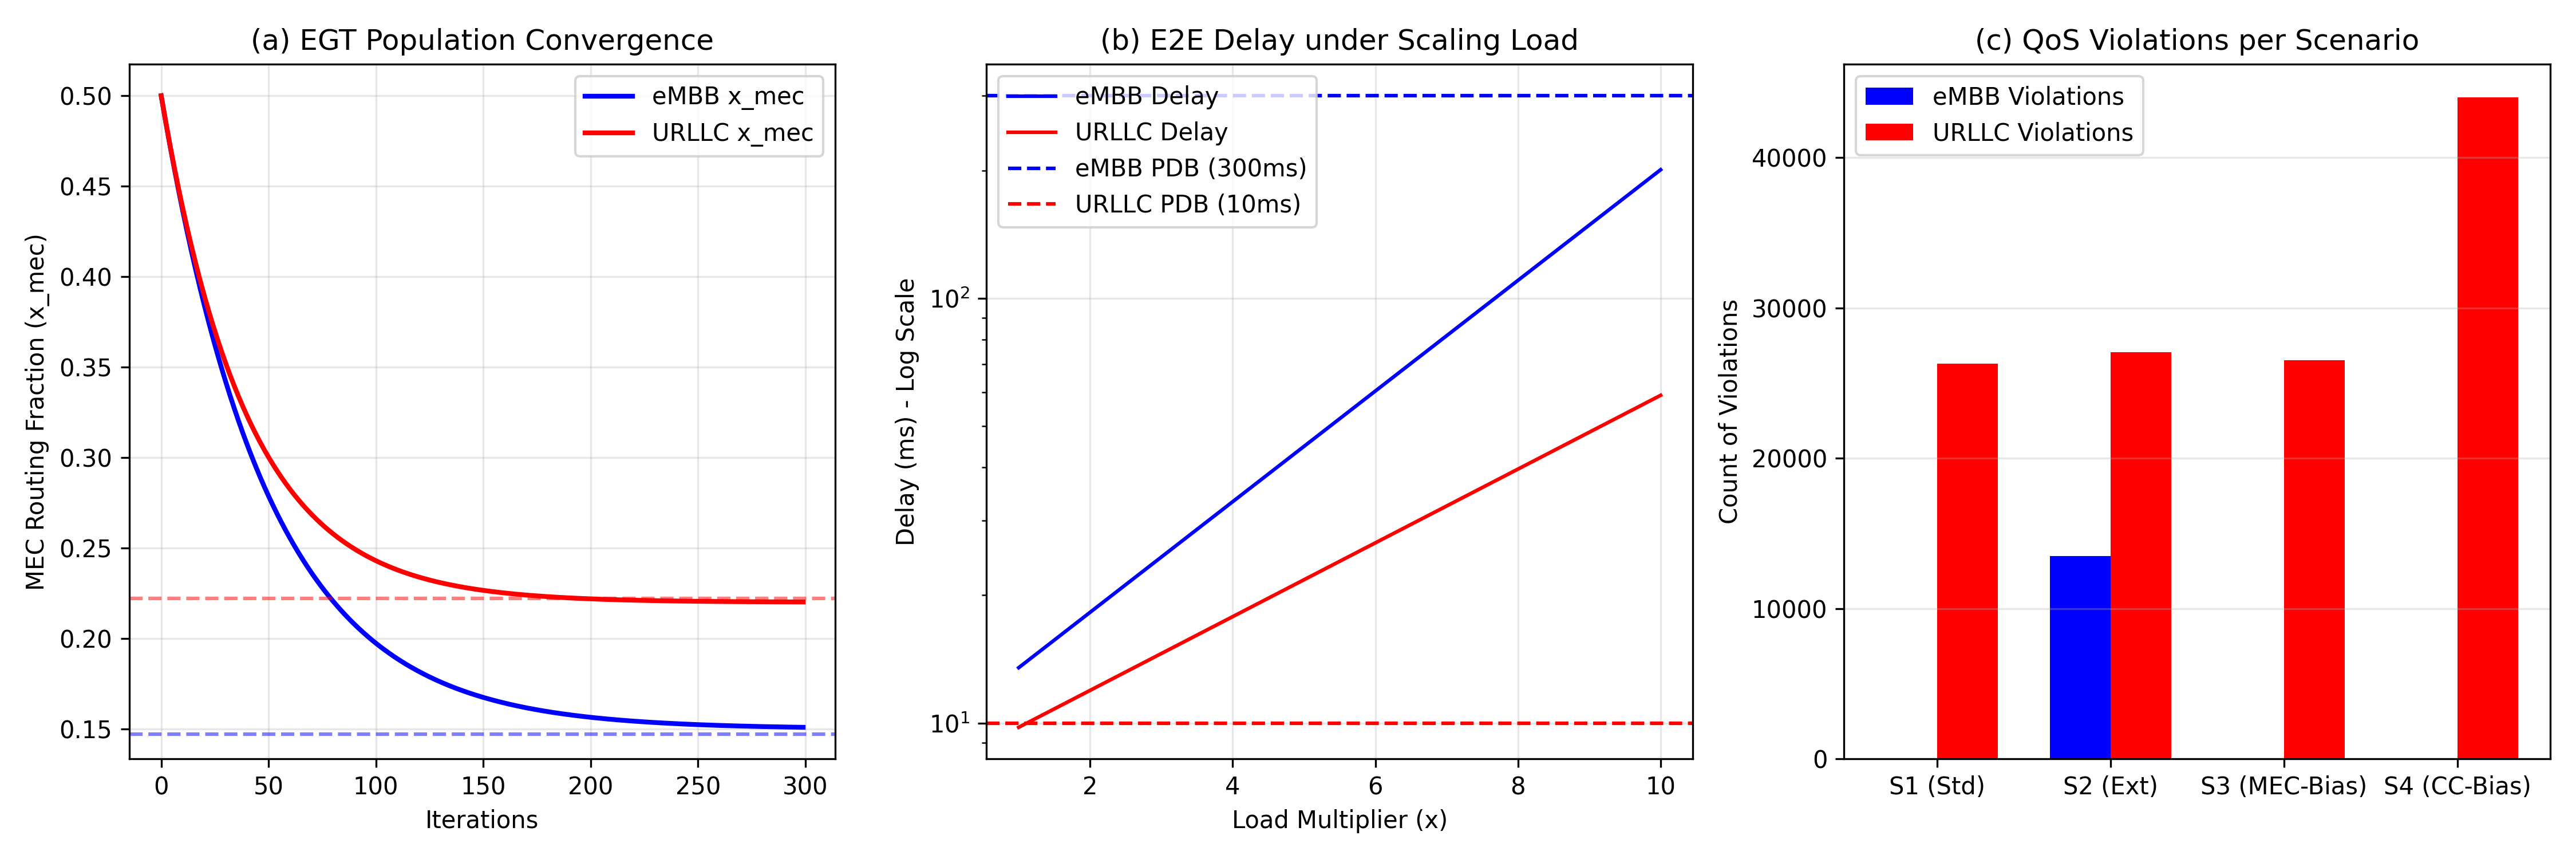
\includegraphics[width=0.95\textwidth]{multi_scenario_1000ue}
    \caption{Emulation results for 1,000 UEs across four scenarios:
    (a) population fractions converging to Nash equilibrium,
    (b) end-to-end delays versus PDB thresholds, and
    (c) throughput and QoS violations.}
    \label{fig:results}
\end{figure*}

%--------------------------------------------------------------
\subsection{Key Analysis and Findings}
\label{sec:key_findings}
%--------------------------------------------------------------

\textbf{Nash equilibrium and delay equalisation.}
In S1, the EGT controller converges to
$x_\text{mec}^\text{eMBB} = 0.156$ and
$x_\text{mec}^\text{URLLC} = 0.222$, routing 12.9~Gbps to the
edge node and 58.6~Gbps to the central cloud. At this equilibrium,
the eMBB end-to-end delays are 27.9~ms (MEC) and 17.9~ms (CC),
yielding a weighted average of 19.5~ms. URLLC delays are 19.5~ms
(MEC) and 17.9~ms (CC), weighted average 18.3~ms. The residual
$\Delta d = 10.0$~ms gap between MEC and CC at the stopping
criterion is the expected numerical consequence of the payoff
convergence tolerance $\varepsilon = 0.01$, not a failure of
the replicator dynamics. Note that the Nash equilibrium equalises
payoffs (inverse delays) rather than delays themselves; as a
result, at the stopping criterion MEC delay exceeds CC delay,
which is the correct outcome given the heavier MEC processing
penalty at this load point.

% R5-Q1: Reworded the URLLC ceiling paragraph to clarify that
%         4.7 Gbps marks where violations BEGIN, not a routing cap
% R6-Q3: Corrected ceiling paragraph: replaced "vastly exceeds" with precise 17.1%
%         threshold; added explanation of why EGT cannot route 0% to MEC (NE dynamics).
\textbf{URLLC infrastructure ceiling.}
At the S1 peak equilibrium, both MEC and CC delays
(19.5~ms and 17.9~ms respectively) exceed the 10~ms URLLC PDB,
resulting in 26,316 violations across the 27,000 URLLC UE-steps
of Phase~II --- a 97.5\% violation rate. This is not a policy
failure but a fundamental infrastructure constraint. From
Eq.~\eqref{eq:upf_delay_mec}, the 4.7~Gbps ceiling identifies
the minimum MEC URLLC load at which PDB$_2$ violations begin:
specifically, the load threshold at which MEC processing delay
reaches exactly $\text{PDB}_2 - t_{\text{prop}_\text{mec}}
= 10 - 0.25 = 9.75$~ms, obtained by solving:
\begin{equation*}
  k_\text{mec} \cdot \rho_\text{URLLC} \cdot M_2 \cdot
  x_\text{mec}^\text{URLLC} \cdot \lambda \;=\; \ln(9.75)
\end{equation*}
giving an effective URLLC load ceiling of approximately 4.7~Gbps
at the MEC node. Any MEC routing fraction above 17.1\% breaches
this ceiling at $5.5\times$ load; the EGT equilibrium fraction
(22.2\%) corresponds to a 6.1~Gbps MEC load --- 30\% above this
threshold. While routing zero fraction to MEC would mathematically
avoid MEC-side violations, the replicator dynamics preclude this:
at $x_\text{mec}=0$, the unloaded MEC node offers payoff
$u_\text{mec}=0.80$ versus $u_\text{cc}=0.031$ for the saturated
CC, driving sessions back to MEC until the interior Nash
equilibrium is reached. The ceiling breach is therefore
structurally enforced by the Nash equilibrium itself.
No steering algorithm can resolve a violation whose root cause
is hardware processing capacity. Future network planning must
treat this derived ceiling as a hard infrastructure dimensioning
constraint.

\textbf{eMBB QoS compliance.}
Zero eMBB violations are recorded in S1, S3, and S4, confirming
that the 19.5~ms weighted average delay is well within the
300~ms eMBB PDB. The EGT controller effectively steers eMBB
traffic toward $\text{UPF}_\text{cc}$ during load surges,
preserving the edge node for delay-sensitive traffic. The 10:1
cloud-to-edge processing exponent ratio ($k_\text{mec}/k_\text{cc}
= 10$) drives sufficient eMBB spillover to the central cloud to
prevent the edge node from saturating for this slice class.

\textbf{Transient recovery, $\varepsilon$-boundaries, and S4.}
All three scenarios S1, S3, and S4 target the same interior Nash
equilibrium under identical offered load. The different reported
equilibrium fractions in Table~\ref{tab:stadium_results} (e.g.\
$x_\text{mec}^\text{eMBB} = 0.156$ for S1 vs.\ $0.128$ for S4)
arise from the discrete $\varepsilon = 0.01$ stopping criterion:
trajectories approaching the Nash point from opposite sides of
the state space halt on opposite edges of the $\varepsilon$-ball.
The scenarios differ in convergence speed: S3 (MEC-Biased
Initialisation, 90\% MEC start) requires 670~iterations, while
S4 (CC-Biased Initialisation, 5\% MEC start) converges in
270~iterations. S4's faster convergence does not imply fewer
violations. Starting at 95\% CC occupancy, the aggregate CC
processing load at Phase~II onset is $0.95 \times 71.5~\text{Gbps}
= 67{,}925~\text{Mbps}$, producing
$t_\text{CC} = \exp(k_\text{cc} \times 67{,}925)
= \exp(3.282) \approx 26.6$~ms processing delay plus
$t_{\text{prop}_\text{cc}} = 1.0$~ms, totalling 27.6~ms ---
well in excess of the 10~ms URLLC PDB. Every URLLC session on the
CC violates the PDB from step one of Phase~II.
% R5-Q3: Corrected S4 violation count reporting — denominator is 57,000 (all 285 steps),
%         not 27,000 (Phase II only), yielding a 77.2% violation rate
Furthermore, S4's 95\% CC-bias under elevated Phase~I load
($\lambda$: 0.509 to 5.0$\times$) produces 16,963 URLLC violations
in Phase~I alone (94.2\% of 18,000 Phase~I UE-steps), before
Phase~II begins. Across all 285 simulation steps (57,000 URLLC
UE-steps), S4 accumulates 44,027 cumulative violations --- a
77.2\% violation rate --- driven by the severe CC-overload
transient before equilibrium is reached and the Phase~I penalty
from the biased initialisation.

\textbf{S2: extreme spike and warm-start tracking.}
Scenario S2 ($10\times$ load, 130~Gbps total) illustrates a
practically important empirical property of EGT replicator
dynamics under sudden extreme load transitions.
When EGT is initialised from a neutral state ($x = 0.5$) and
converged in a single cold-start call at $10\times$ load with
$\varepsilon = 0.01$, the optimiser converges in 213 iterations
to the all-MEC boundary equilibrium ($x_\text{mec} = 1.0$),
where the payoff equality condition is trivially satisfied at
zero CC occupancy. An intermediate snapshot at approximately
iteration 150 shows $x_\text{mec}^\text{eMBB} \approx 0.380$,
producing catastrophic MEC processing delay
($d_\text{eMBB}^\text{MEC} \approx 2.4\times10^6$~ms), but the
algorithm proceeds to the boundary rather than halting there.
While physical UPFs would drop packets rather than queue them
indefinitely, this boundary-convergence behaviour demonstrates
that cold-start EGT fails to find a safe routing trajectory
under massive initial disruption, underscoring the practical
necessity of warm-start tracking.
The true Nash equilibrium at $10\times$
load (reachable only by tightening $\varepsilon$ to $10^{-5}$,
requiring 7,673 iterations) lies at
$x_\text{mec}^\text{eMBB} \approx 0.136$ with an average
delay of 188.8~ms.

In the actual stadium simulation, EGT operates in continuous
warm-start tracking mode, as illustrated in
Fig.~\ref{fig:flowchart_dispatch}, stepping through the load
trajectory from Phase~I. When Phase~II begins, the population
state is already close to the active equilibrium
($x_\text{mec}^\text{eMBB} \approx 0.229$ at Phase~I end).
EGT progressively migrates traffic across the 135 Phase~II
timesteps, stabilising at $x_\text{mec}^\text{eMBB} = 0.147$
with a MEC load of 23.8~Gbps. Cumulative eMBB violations
total 13,491, confined exclusively to Phase~II (confirmed
zero violations in Phases~I and~III); these represent only
the transient steps during active migration.
Phase~III generates a small residual of 597 URLLC violations
during the dispersal transient as load ramps from $\lambda
\approx 9.0\times$ down to $0.3\times$ (S2-specific dispersal
profile; see Table~\ref{tab:scenario_def}).
% R5-Q6 / R6-Q7 / R7-Q1: Updated per-step iteration distribution to clearly attribute
%                 S1 (max=122) and S2 (max=147) statistics separately.
Per-step re-convergence under warm-start tracking requires
as few as 1~iteration per step under standard load conditions.
Under S1 conditions (5.5$\times$ load), 131 of 135
Phase~II timesteps (97\%) converge in exactly 1 replicator
iteration; the remaining 4 steps require 21--122 iterations
at load-transition boundaries (mean: 3.3 iterations/step,
median: 1). By contrast, the 505 iterations reported in Table~II
represent a theoretical cold-start benchmark from a neutral state.
Under the extreme 10$\times$ surge (S2), 133 of 135
Phase~II steps (98.5\%) converge in 1 iteration; the maximum
of 147 iterations occurs at a single load-transition step.
This confirms that continuous warm-start tracking
avoids the cold-start numerical trap, an empirically
demonstrated advantage of step-by-step dynamic EGT.

\textbf{Baseline comparison.}
% R5-Q7: Added sentence explaining 20/80 static alternative still violates;
%         clarified that 50/50 is the OAI zero-configuration default
Under static 50/50 routing, 35.8~Gbps is steered to the MEC
node, driving average eMBB MEC delay to
$\approx 4.15\times10^4$~ms and average URLLC MEC delay to
$769$~ms. The central cloud, receiving an equal 35.8~Gbps,
remains lightly loaded at 6.6~ms. The weighted average eMBB
delay is 20,736~ms and URLLC average is 388~ms, both far
exceeding their PDB targets. The 50/50 split was chosen as the
zero-configuration OAI default, representing the failure mode
of the most naive deployment. A static 20/80 split would reduce
MEC URLLC load to 5.5~Gbps (still 17\% above the 4.7~Gbps
ceiling), sustaining near-total URLLC violations while
catastrophically overloading MEC eMBB traffic --- confirming
that no static policy can resolve the infrastructure ceiling
at $5.5\times$ load. This confirms that static routing
catastrophically overloads the edge node while leaving the
cloud idle, whereas the EGT controller converges to a
% R6-Q10: Replaced "jointly optimal operating point" with accurate Nash-stable description.
%          The NE is Pareto-dominated by a centralised optimal split (3.5% aggregate delay
%          reduction), so "jointly optimal" is incorrect.
Nash-stable operating point that is strictly superior to static
routing for both slices simultaneously --- though it is not a
social welfare optimum, as a centralised optimiser could reduce
aggregate delay by a further 3.5\% at the cost of increasing
URLLC MEC delay by 5~ms.

\section{Future Work}
\label{sec:future}

The validated EGT steering logic opens several avenues
for future research.

\subsection{PDB-Aware Payoff Function}

The most critical near-term enhancement is the replacement
of the current delay-minimising payoff $u = 1/d$ with a
PDB-margin payoff of the form
$u_i^g = \text{PDB}_g / d_i^g(\mathbf{x},\lambda)$.
This slice-aware formulation weights UPF strategies by their
margin relative to the per-slice PDB threshold rather than raw
delay, driving URLLC traffic more aggressively toward
lower-delay nodes and potentially reducing the transient
violation count under load surges.

\subsection{Predictive ML-Based Reconfiguration Triggers}

A further enhancement is the transition from periodic
scheduling to an event-driven reconfiguration trigger.
We propose the integration of a Bidirectional LSTM
(BLSTM) model within the EGT control loop. Trained on
mobility-driven QoS degradation traces, this model
would utilise three primary indicators---the
reconfiguration countdown $T_g^{\text{reconf}}$, the
predicted session violation time $T_{g}^{\text{vio}}$,
and the instantaneous violation count $L_a$---to
proactively initiate EGT re-convergence before
violations occur, following the approach of~\cite{LeyvaUPC2023}.

\subsection{Economic and OPEX-Aware Optimisation}

Future work will address the operational cost dimension
of edge steering. MEC resources are typically more
expensive to maintain than centralised cloud infrastructure.
We plan to extend the payoff function $u(\mathbf{x})$
to include an economic weight factor that penalises
edge strategies for non-critical traffic, enabling
operators to reserve premium MEC capacity for URLLC
slices while directing eMBB traffic to more
cost-effective cloud resources during low-congestion
periods.

\subsection{Sustainability and Energy-Aware Steering}

In alignment with Green-6G objectives, we intend to
incorporate power consumption models into the steering
logic. Since distributed edge UPFs can consume more
energy per bit than consolidated cloud data centres, an
energy-aware orchestration layer could adjust the EGT
equilibrium to enable reduced-power states for local
UPFs during the post-event dispersal phase, balancing
latency performance against the venue's overall energy
footprint.

\subsection{Validation on Physical Testbeds}

Further experimental validation is required using
NSSF-enabled dual-UPF deployments in physical testbeds,
with real over-the-air radio rather than emulated UE
sessions. Investigating the impact of control-plane
signalling overhead during mass PDU session establishment
events remains a high priority for hardware-in-the-loop
studies.

\section{Conclusion}

This paper has presented a slice-aware, dual-UPF
selection framework for 5G stadium environments,
integrating Evolutionary Game Theory (EGT) replicator
dynamics within the SMF with an OpenAirInterface (OAI)
emulation testbed. The OAI testbed validated session
scalability, achieving 100\% PDU session establishment
success for 1,000 concurrent UE contexts via a
high-performance Go-based user-plane multiplexing engine.
QoS performance was evaluated using an analytical queuing
model calibrated against published results.

% R6-Q5, R7-Q2: Corrected first finding — zero eMBB violations only for S1/S3/S4;
%         S2 has 12.5% violation rate across Phase II UE-steps.
The key findings are threefold. First, the EGT-based
steering achieves zero eMBB QoS violations across all
standard and initialisation-variant scenarios (S1, S3, S4)
by exploiting the 10:1 cloud-to-edge processing exponent
ratio. In the extreme 10$\times$ stress scenario S2, eMBB
violations affect 12.5\% of Phase~II UE-steps
during active migration and cease at convergence.
Second, the EGT controller converges to a stable equilibrium across all
evaluated scenarios: theoretical static cold-starts require
270--670~iterations depending on initialisation
conditions, while continuous warm-start tracking
% R6-Q7: Correctly attribute iteration ranges per scenario
resolves in as few as 1~iteration per step under
standard load (S1: max 122 iterations at load-transition
boundaries) and up to 147~iterations per step during the
extreme $10\times$ load surge (S2: single isolated step),
consistent with the convergence guarantees of~\cite{Alevizaki2021upf}.
Third, and most critically, the study identifies a hard
infrastructure ceiling for URLLC QoS compliance: at the
5.5$\times$ halftime surge, 97.5\% of URLLC UE-steps
violate the 10~ms PDB during Phase~II (26,316 of 27,000
in S1), because the 4.7~Gbps MEC URLLC load ceiling ---
the threshold at which PDB$_2$ violations begin --- is
exceeded by 30\% at the equilibrium routing fraction
(6.1~Gbps). No steering algorithm alone can overcome
this constraint; URLLC PDB guarantees in stadium
deployments require explicit infrastructure
dimensioning alongside algorithmic steering.

Future research will prioritise a PDB-margin payoff
function to improve slice-awareness, BLSTM-based
predictive triggers to reduce reactive reconfiguration
overhead, and physical testbed validation with real
over-the-air traffic.

\bibliographystyle{IEEEtran}
\bibliography{references}

\end{document}
